\documentclass[a4paper,11pt,twoside]{report}
\usepackage{etex}
\usepackage[left=2.5cm,right=2cm,top=2cm,bottom=2cm]{geometry}

\usepackage{graphicx}
\DeclareGraphicsExtensions{.pdf,.jpeg,.jpg}

\usepackage{verbatim}
\usepackage{pgfplots}
\usepackage{latexsym}
\usepackage{mathchars}
\usepackage{setspace}
\usepackage{dirtree}

\usepackage{cleveref} 
\usepackage{color}               %obv
\usepackage{appendix}            %obv
\usepackage{amsmath}             %for math environment
\usepackage{mathtools}

\usepackage{enumitem}            %for modifying lists
\setitemize{noitemsep,topsep=0pt,parsep=0pt,partopsep=0pt}
\setenumerate{noitemsep,topsep=0pt,parsep=0pt,partopsep=0pt}

\usepackage[procnames]{listings} %for inserting code
\usepackage{fancyvrb} % for inserting .txt
\usepackage{parskip}             %for modifying spacing

\usepackage{float}              %for forcefully placing diagrams 
\usepackage[colorlinks=false, pdfborder={0 0 0}]{hyperref}
\usepackage{algorithm}
\usepackage{algpseudocode}
\newcommand{\tab}[1]{\hspace{.08\textwidth}{#1}} % indent tab for data
                                                 % structs in algos
\newcommand{\LineIf}[3]{ {#1}
  \algorithmicif\ {#2}
  \algorithmicelse\ {#3} } % inline X if Y else Z

\usepackage{booktabs}
%\usepackage{subfig}
\usepackage{subcaption}
\usepackage{wrapfig}
\usepackage{floatflt}

\usepackage[backref=true,
  %style=authoryear,
  style=numeric-comp,
  citereset=section,
  maxcitenames=3,
  maxbibnames=100]{biblatex}
\bibliography{thesis}
\DefineBibliographyStrings{english}{%
  backrefpage  = {see p.}, % for single page number
  backrefpages = {see pp.} % for multiple page numbers
}
\setlength\bibitemsep{1em}

\usepackage{titlesec}
\titlespacing\section{0pt}{12pt plus 4pt minus 2pt}{0pt plus 2pt minus 2pt}
\titlespacing\subsection{0pt}{12pt plus 4pt minus 2pt}{0pt plus 2pt minus 2pt}
\titlespacing\subsubsection{0pt}{12pt plus 4pt minus 2pt}{0pt plus 2pt minus 2pt}

\setlength{\parskip}{\medskipamount}  % a little space before a \par
\setlength{\parindent}{0pt}	      % don't indent first lines of paragraphs
%UHEAD.STY  If this is included after \documentstyle{report}, it adds
% an underlined heading style to the LaTeX report style.
% \pagestyle{uheadings} will put underlined headings at the top
% of each page. The right page headings are the Chapter titles and
% the left page titles are supplied by \def\lefthead{text}.

% Ted Shapin, Dec. 17, 1986

\makeatletter
\def\chapapp2{Chapter}

\def\appendix{\par
 \setcounter{chapter}{0}
 \setcounter{section}{0}
 \def\chapapp2{Appendix}
 \def\@chapapp{Appendix}
 \def\thechapter{\Alph{chapter}}}

\def\ps@uheadings{\let\@mkboth\markboth
% modifications
\def\@oddhead{\protect\underline{\protect\makebox[\textwidth][l]
		{\sl\rightmark\hfill\rm\thepage}}}
\def\@oddfoot{}
\def\@evenfoot{}
\def\@evenhead{\protect\underline{\protect\makebox[\textwidth][l]
		{\rm\thepage\hfill\sl\leftmark}}}
% end of modifications
\def\chaptermark##1{\markboth {\ifnum \c@secnumdepth >\m@ne
 \chapapp2\ \thechapter. \ \fi ##1}{}}%
\def\sectionmark##1{\markright {\ifnum \c@secnumdepth >\z@
   \thesection. \ \fi ##1}}}
\makeatother
%%From: marcel@cs.caltech.edu (Marcel van der Goot)
%%Newsgroups: comp.text.tex
%%Subject: illegal modification of boxit.sty
%%Date: 28 Feb 92 01:10:02 GMT
%%Organization: California Institute of Technology (CS dept)
%%Nntp-Posting-Host: andromeda.cs.caltech.edu
%%
%%
%%Quite some time ago I posted a file boxit.sty; maybe it made it
%%to some archives, although I don't recall submitting it. It defines
%%	\begin{boxit}
%%	...
%%	\end{boxit}
%%to draw a box around `...', where the `...' can contain other
%%environments (e.g., a verbatim environment). Unfortunately, it had
%%a problem: it did not work if you used it in paragraph mode, i.e., it
%%only worked if there was an empty line in front of \begin{boxit}.
%%Luckily, that is easily corrected.
%%
%%HOWEVER, apparently someone noticed the problem, tried to correct it,
%%and then distributed this modified version. That would be fine with me,
%%except that:
%%1. There was no note in the file about this modification, it only has my
%%   name in it.
%%2. The modification is wrong: now it only works if there is *no* empty
%%   line in front of \begin{boxit}. In my opinion this bug is worse than
%%   the original one.
%%
%%In particular, the author of this modification tried to force an empty
%%line by inserting a `\\' in the definition of \Beginboxit. If you have
%%a version of boxit.sty with a `\\', please delete it. If you have my
%%old version of boxit.sty, please also delete it. Below is an improved
%%version.
%%
%%Thanks to Joe Armstrong for drawing my attention to the bug and to the
%%illegal version.
%%
%%                                          Marcel van der Goot
%% .---------------------------------------------------------------
%% | Blauw de viooltjes,                    marcel@cs.caltech.edu
%% |    Rood zijn de rozen;
%% | Een rijm kan gezet
%% |    Met plaksel en dozen.
%% |


% boxit.sty
% version: 27 Feb 1992
%
% Defines a boxit environment, which draws lines around its contents.
% Usage:
%   \begin{boxit}
%	... (text you want to be boxed, can contain other environments)
%   \end{boxit}
%
% The width of the box is the width of the contents.
% The boxit* environment behaves the same, except that the box will be
% at least as wide as a normal paragraph.
%
% The reason for writing it this way (rather than with the \boxit#1 macro
% from the TeXbook), is that now you can box verbatim text, as in
%   \begin{boxit}
%   \begin{verbatim}
%   this better come out in boxed verbatim mode ...
%   \end{verbatim}
%   \end{boxit}
%
%						Marcel van der Goot
%						marcel@cs.caltech.edu
%

\def\Beginboxit
   {\par
    \vbox\bgroup
	   \hrule
	   \hbox\bgroup
		  \vrule \kern1.2pt %
		  \vbox\bgroup\kern1.2pt
   }

\def\Endboxit{%
			      \kern1.2pt
		       \egroup
		  \kern1.2pt\vrule
		\egroup
	   \hrule
	 \egroup
   }	

\newenvironment{boxit}{\Beginboxit}{\Endboxit}
\newenvironment{boxit*}{\Beginboxit\hbox to\hsize{}}{\Endboxit}
\input{icthesis.sty}
%\usepackage{algorithm2e}

\newcommand{\ipc}{{\sf ipc}}

\newcommand{\Prob}{\bbbp}
\newcommand{\Real}{\bbbr}
\newcommand{\real}{\Real}
\newcommand{\Int}{\bbbz}
\newcommand{\Nat}{\bbbn}

\newcommand{\NN}{{\sf I\kern-0.14emN}}   % Natural numbers
\newcommand{\ZZ}{{\sf Z\kern-0.45emZ}}   % Integers
\newcommand{\QQQ}{{\sf C\kern-0.48emQ}}   % Rational numbers
\newcommand{\RR}{{\sf I\kern-0.14emR}}   % Real numbers
\newcommand{\KK}{{\cal K}}
\newcommand{\OO}{{\cal O}}
\newcommand{\AAA}{{\bf A}}
\newcommand{\HH}{{\bf H}}
\newcommand{\II}{{\bf I}}
\newcommand{\LL}{{\bf L}}
\newcommand{\PP}{{\bf P}}
\newcommand{\PPprime}{{\bf P'}}
\newcommand{\QQ}{{\bf Q}}
\newcommand{\UU}{{\bf U}}
\newcommand{\UUprime}{{\bf U'}}
\newcommand{\zzero}{{\bf 0}}
\newcommand{\ppi}{\mbox{\boldmath $\pi$}}
\newcommand{\aalph}{\mbox{\boldmath $\alpha$}}
\newcommand{\bb}{{\bf b}}
\newcommand{\ee}{{\bf e}}
\newcommand{\mmu}{\mbox{\boldmath $\mu$}}
\newcommand{\vv}{{\bf v}}
\newcommand{\xx}{{\bf x}}
\newcommand{\yy}{{\bf y}}
\newcommand{\zz}{{\bf z}}
\newcommand{\oomeg}{\mbox{\boldmath $\omega$}}
\newcommand{\res}{{\bf res}}
\newcommand{\cchi}{{\mbox{\raisebox{.4ex}{$\chi$}}}}
%\newcommand{\cchi}{{\cal X}}
%\newcommand{\cchi}{\mbox{\Large $\chi$}}

% Logical operators and symbols
\newcommand{\imply}{\Rightarrow}
\newcommand{\bimply}{\Leftrightarrow}
\newcommand{\union}{\cup}
\newcommand{\intersect}{\cap}
\newcommand{\boolor}{\vee}
\newcommand{\booland}{\wedge}
\newcommand{\boolimply}{\imply}
\newcommand{\boolbimply}{\bimply}
\newcommand{\boolnot}{\neg}
\newcommand{\boolsat}{\!\models}
\newcommand{\boolnsat}{\!\not\models}

\newcommand{\op}[1]{\mathrm{#1}}
\newcommand{\s}[1]{\ensuremath{\mathcal #1}}

% Properly styled differentiation and integration operators
\newcommand{\diff}[1]{\mathrm{\frac{d}{d\mathit{#1}}}}
\newcommand{\diffII}[1]{\mathrm{\frac{d^2}{d\mathit{#1}^2}}}
\newcommand{\intg}[4]{\int_{#3}^{#4} #1 \, \mathrm{d}#2}
\newcommand{\intgd}[4]{\int\!\!\!\!\int_{#4} #1 \, \mathrm{d}#2 \, \mathrm{d}#3}

% Large () brackets on different lines of an eqnarray environment
\newcommand{\Leftbrace}[1]{\left(\raisebox{0mm}[#1][#1]{}\right.}
\newcommand{\Rightbrace}[1]{\left.\raisebox{0mm}[#1][#1]{}\right)}

% Funky symobols for footnotes
\newcommand{\symbolfootnote}{\renewcommand{\thefootnote}{\fnsymbol{footnote}}}
% now add \symbolfootnote to the beginning of the document...

\newcommand{\normallinespacing}{\renewcommand{\baselinestretch}{1.5} \normalsize}
\newcommand{\mediumlinespacing}{\renewcommand{\baselinestretch}{1.2} \normalsize}
\newcommand{\narrowlinespacing}{\renewcommand{\baselinestretch}{1.0} \normalsize}
\newcommand{\bump}{\noalign{\vspace*{\doublerulesep}}}
\newcommand{\cell}{\multicolumn{1}{}{}}
\newcommand{\spann}{\mbox{span}}
\newcommand{\diagg}{\mbox{diag}}
\newcommand{\modd}{\mbox{mod}}
\newcommand{\minn}{\mbox{min}}
\newcommand{\andd}{\mbox{and}}
\newcommand{\forr}{\mbox{for}}
\newcommand{\EE}{\mbox{E}}

\newcommand{\deff}{\stackrel{\mathrm{def}}{=}}
\newcommand{\syncc}{~\stackrel{\textstyle \rhd\kern-0.57em\lhd}{\scriptstyle L}~}

\def\coop{\mbox{\large $\rhd\!\!\!\lhd$}}
\newcommand{\sync}[1]{\raisebox{-1.0ex}{$\;\stackrel{\coop}{\scriptscriptstyle
      #1}\,$}}

\newtheorem{definition}{Definition}[chapter]
\newtheorem{theorem}{Theorem}[chapter]

\newcommand{\Figref}[1]{Figure~\ref{#1}}
\newcommand{\fig}[3]{
  \begin{figure}[!ht]
    \begin{center}
      \scalebox{#3}{\includegraphics{figs/#1.ps}}
      \vspace{-0.1in}
      \caption[ ]{\label{#1} #2}
    \end{center}
  \end{figure}
}

\newcommand{\figtwo}[8]{
  \begin{figure}
    \parbox[b]{#4 \textwidth}{
      \begin{center}
        \scalebox{#3}{\includegraphics{figs/#1.ps}}
        \vspace{-0.1in}
        \caption{\label{#1}#2}
      \end{center}
    }
    \hfill
    \parbox[b]{#8 \textwidth}{
      \begin{center}
        \scalebox{#7}{\includegraphics{figs/#5.ps}}
        \vspace{-0.1in}
        \caption{\label{#5}#6}
      \end{center}
    }
  \end{figure}
}


\usepackage{tikz}
\usetikzlibrary{shapes,
  arrows,
  chains,
  matrix,
  positioning,
  fit,
  scopes,
  calc,
  decorations.pathmorphing}
\makeatletter
\tikzset{join/.code=\tikzset{after node path={%
\ifx\tikzchainprevious\pgfutil@empty\else(\tikzchainprevious)%
edge[every join]#1(\tikzchaincurrent)\fi}}}
\makeatother
\tikzset{>=stealth',every on chain/.append style={join},
         every join/.style={->},
         snake it/.style={decorate, decoration=snake}}
\tikzstyle{labeled}=[execute at begin node=$\scriptstyle,
   execute at end node=$]

\tikzset{ 
  table/.style={
    matrix of nodes,
    row sep=-\pgflinewidth,
    column sep=-\pgflinewidth,
    nodes={rectangle,draw=black,text width=3ex,align=center},
    text depth=0.5ex,
    text height=2ex,
    nodes in empty cells
  },
  texto/.style={font=\large\sffamily},
  title/.style={font=\large\sffamily}
}


\newcommand\CellText[2]{%
  \node[texto,left=of mat#1,anchor=east]
  at (mat#1.west)
  {\large #2};
}

\newcommand\SlText[2]{%
  \node[texto,left=of mat#1,anchor=west,rotate=50]
  at ([xshift=1.5ex,yshift=1ex]mat#1.north)
  {\large #2};
}

\newcommand{\super}[1]{\textsuperscript{#1}}

%% \renewcommand{\cite}[1]{\footcite{#1}}

\definecolor{keywords}{RGB}{255,0,90}
\definecolor{comments}{RGB}{0,0,113}
\definecolor{red}{RGB}{160,0,0}
\definecolor{green}{RGB}{0,150,0}
\lstset{frame=tb,
  language=Python,
  aboveskip=3mm,
  belowskip=3mm,
  showstringspaces=false,
  columns=flexible,
  basicstyle={\small\ttfamily},
  numbers=none,
  numberstyle=\tiny\color{gray},
  keywordstyle=\color{keywords},
  commentstyle=\color{comments},
  stringstyle=\color{red},
  breaklines=true,
  breakatwhitespace=true,
  tabsize=3,
  procnamekeys={def,class}
}


\definecolor{deepblue}{HTML}{193441}
\definecolor{navyblue}{HTML}{3e606F}
\definecolor{bluegreen}{HTML}{91AA9D}
\definecolor{beige}{HTML}{D1DBBD}
\definecolor{cream}{HTML}{FCFFF5}

\definecolor{blue}{HTML}{3e606F}
\definecolor{green}{HTML}{91AA9D}

\definecolor{redi}{RGB}{255,38,0}
\definecolor{yellowi}{HTML}{D1DBBD}
\definecolor{greeni}{HTML}{91AA9D}

\newenvironment{itemize*}%
               {\begin{itemize}%
                   \setlength{\itemsep}{0pt}%
                   \setlength{\parskip}{0pt}}%
               {\end{itemize}}
\newenvironment{description*}%
               {\begin{description}%
                   \setlength{\itemsep}{0pt}%
                   \setlength{\parskip}{0pt}}%
               {\end{description}}



\def \mheight {1cm}
\def \mwidth {1cm}
\definecolor{col2}{HTML}{C7BA9B}
\definecolor{col1}{HTML}{8B7C6D}
\definecolor{col3}{HTML}{F0EAB3}
\definecolor{col4}{HTML}{626072}
\definecolor{col5}{HTML}{40415B}

\tikzstyle{bx}=[
  fill, 
  minimum height=\mheight, 
  minimum width=\mwidth, 
  shape border rotate=90, 
  shape aspect=0.1,
  rounded corners=2mm
]

\tikzstyle{cld}=[
  cloud, 
  cloud puffs=15.7, 
  cloud ignores aspect, 
  minimum height=\mheight,
  minimum width=\mwidth, 
  align=center
]

\tikzstyle{dtb}=[
  fill,
  chamfered rectangle,
  chamfered rectangle xsep=2cm,
  minimum height=\mheight, 
  minimum width=\mwidth,
  rounded corners=1mm
]


\begin{document}

\title{\LARGE {\bf Inside Wikipedia: Analysing articles, edits and editors}\\
 \vspace*{6mm}
}

\author{William Marsey}
\submitdate{5 September 2014}

\normallinespacing
\maketitle

\preface
\addcontentsline{toc}{chapter}{Abstract}

\begin{abstract}
In this project, we analyse Wikipedia revision histories, with a view
to automatically deriving an collaborative share for each of the
article's editors. We use automatic, semantically-na\"ive string
analysis as a basis for discussing the value of each contribution in
an article's history. We analyse the edit distance between texts in
various ways, and, in particular, try to characterise the each step of
an article's path as connected to, completely contextualised by, every
other in that history.

It strikes us that, as a Wikipedia article is something that evolves
organically out of the actions of many competing agents, then we may
measure the success of a contribution -- the smallest unit of which is
a character -- to be it's survival rate. Other studies have remarked
upon this also. However, previous studies that endeavour to
characterise or measure this survival rate concentrate on identifying
binary do/undo interaction between edits, which -- as we'll see -- is
a common occurence, but we feel is inadequate in terms of really
understanding the constant, nuanced to-and-fro of mass online
collaboration. We offer a solution in our `trajectory' technique.

We also spend time exploring value in the fact of the edit itself --
may we evaluate an edit according to it's actual content? We consider
the text as composed of numerous different species of text, dividing
it using Wikipedia's native markup convention, `wikimarkup', and look
to find correlations between text species and survival rate. Indeed
this project follows one that did only this, and most of the time
spent on this project was automating and exploring this approach.

We find that, on Wikipedia in particular, that qualitative analysis of
text, at least characterised by species in this way, does not
correlate well to survival, and thus to any kind of Wikipedia-native
`quality'. We also discuss complicating external factors.

Though this observation may render a fair amount of the text-analysis
work obsolete in the case of analysing Wikipedia in particular, the
produced software is robust and malleable, and the procedures
developed and implemented here would lend themselves well to analysing
the interaction-driven analystical paradigm formerly
aforementioned. As it stands, this work would adapt well to analysis
of more stable forms of online contribution, such as source control
models. We end by discussing and demonstrating the prospects of these
possible extensions.
\end{abstract}

%% \cleardoublepage

\addcontentsline{toc}{chapter}{Acknowledgements}

\begin{acknowledgements}

I would like to express (whatever feelings I have) to:

\begin{itemize}
 \item My supervisor
 \vspace*{3mm}
 \item My second supervisor
 \vspace*{3mm}
 \item Other researchers
 \vspace*{3mm}
 \item My family and friends
\end{itemize}

\end{acknowledgements}
%% \cleardoublepage

\begin{dedication}
  Dedication here.
\end{dedication}
\clearpage

\narrowlinespacing

\vspace*{4mm}

``This page documents \ldots a generally accepted standard that
editors should follow, though it should be treated with common sense,
and occasional exceptions may apply. Changes made to it should reflect
consensus; when in doubt, discuss your idea on the talk page.''

``Once an article reaches the A-Class, it is considered ``complete'',
although edits will continue to be made.''

from \emph{Wikipedia:Version 1.0 Editorial Team/Assessment, en.wikipedia.org}
\normallinespacing


\body
\chapter{Introduction}
\label{ch:introduction}
\section{Objectives}
Our principal aim was to design a series of procedures for
distributing a `share' of a collaborative article to each of that
article's contributors. Traditionally these shares are negotiated --
in an opera commission, for instance, various stakes in the work will
be distributed and defined according to negotations, between
individuals, or corporations; between a composer's and a librettist's
agents, or between the individuals personally, also taking into
account comissioner's rights, and other things. Our investigation
instead looks to automatic share distribution in the environment of
many-user online collaboration; how may we automatically define a
individual user's stake in a collobaritive work?

Wikipedia is the natural choice for the study, though defining user
`ownership' in this particular context seems quite unnatural -- the
website that bills itself as the `free encyclopedia that anyone can
edit' can hardly have any obligation to its users to define a sense of
individual ownership of the article, whole or otherwise. However, as
an intellectual exercise, the question seems very important. 

The technological platforms that allow projects such as Wikipedia to
grow also open up the opportunity for study. Using the technology, we
may may examine how to describe the nature of an individual
contribution amongst many -- a question that, in the context of
growing popularity of crowd-sourcing information, seems
pertinent. Wikipedia is, after all, one of the most popular sites on
the internet, and certainly one the most popular reference site on the
internet.

On a more general level, Wikipedia represents a free, flexible and
(fairly) complete data set with which to experiment analysing text
change over long periods. From this base work we can begin to approach
analysing more specific data sets, such as source-control.

Another benefit of analysing Wikipedia is that interactions between
wholly mediated by the Wikipedia software, and evidenced in exactly
the same way the actual data is, allowing us to examine a relatively
wide range of site properties using the same tools.

In this project, we produce a system for automatically grabbing an
article's history, along with various methods with which to
characterise that data. We use a Levenshtein edit-distance calculating
algorithm in order to examine the magnitude of change between edits,
as well as to examine the context of those edits.

For each revision we calculate a set of integers that represent a
multi-dimension characterisation of the change that edit caused in the
article. We provide other means to express the degree to which that
edit was significant in terms of the history of that article thus far.

%% Despite early skepticism (particularly concern over the inherent chaos
%% in the system: ``...edits, contributed in a predominantly undirected
%% and haphazard fashion by ... unvetted
%% volunteers.''\cite{Wilkinson2007}), Wikipedia is widely claimed to be
%% a great success, `the best-developed attempt thus far of the enduring
%% quest to gather all human knowledge in one
%% place'\cite{Mesgari2014}. The website is only around a decade old, but
%% in that time it has become a pre-eminent source of knowledge one the
%% internet. As a highly populous, visible and accessible online space,
%% the site is 

%% It is one of the most visited sites in the world, and the
%% most visited reference site by far. It is a huge site, with over 4.5
%% million article, in around 300 language languages, and is completely
%% open source and free-of-charge. It is an unparalleled data source,
%% detailed and easy to access.

%% However, one of the major factors contributing to the proliferation of
%% academic work on wikipedia is suspicion. Investigations into the worth
%% and quality of Wikipedia articles abound. Work in this area ranged
%% from popular science to production software to full-blown academic
%% theses, and until around 2010 continued to be a well-visited topic.

%% In recent years, however, the research into wikipedia's extrinsic
%% quality has waned. These studies peaked at around 2007, in the release
%% of the Wikitrust software, which brought together much of the
%% preceding researh on the subject, and is discussed later. Since then,
%% though, papers on Wikipedian quality became less frequent, and
%% Wikipedia reached real omnipresence.  In these years, while the fears
%% that these crowd-sourced articles would supercede established
%% reference tomes were certainly realised, so did the public seem to
%% maintain a healthy suspicion of the site. Wikipedia is a central point
%% of fact-checking, with even search tools such as Google's voice search
%% and Apple's Siri taking it's content for granted, serving up
%% Wikipedian content automatically after voice searches, but the site is
%% still not accepted as a citable source.

%% Criticisms of Wikipedia still exists, however. Though, whilst they
%% began as investigations into external quality, now they more often
%% than not concern Wikiepdia's internal health. We can no longer argue
%% about whether or not the public should be reading these articles --
%% they already are. Instead, we examine the internals of Wikipedia, and
%% into the community that is involved in its growth. 

%% This is the context for our study. We can assume that an article has
%% worth, we don't care what that might be. We look at how this
%% may be distributed within the article. What can we find out about the
%% article by examining it's construction? What can we automatically
%% measure of a revision's text?

%% The objective of this project was to find a fair and concise way to
%% analyse a Wikipedia revision, both in terms of the text operations,
%% and in terms of an edits significance in the overall history of the
%% article.

\section{Contributions}

The major contribution here is a new way of visualising the article's
history, and a technique for translating that into a meaningful value
for each revision. 

We also discuss using the software developed here to achieve various
other contexts relating to the journey of each article. Our main
technique involves calculating the similarity of every revision to the
final version. However, using the same software we may also track the
history of the talk page for each article alongside the article
itself, as well as test for the existence of `arbritration requests'
and other artefacts of Wikipedian bureaucracy that come to bear on the
circumstances that control an article's development. 

The software produced here automates the processing of the analytical
procedures we outline later, as well as providing a modular framework
to be modified for further study.

\section{Originality}
There has been a lot of studies tangential to the topics we discuss
here -- as we'll cover later, Wikipedia is a hotbed of many avenues of
academic study -- but much of the similar work to this works to
different ends, and therefore a lot of the work here is original work.

The most related work is that of WikiTrust software. It was developed
in the context of criticism's of Wikipedia's factual integrity, and
aimed to rate the the editors of each article, transforming each
article into a kind of heat map or trustability, highlighting words
from more trusted editors more intensely than others. 

We offer less judgments on quality in this project, and our aims are
more general, but some of the techniques resurface here. In
particular, we modify the WikiTrust method for identifying undone work
to create a much more detailed flow of change.

This project was also undertaken for the MSc degree at Imperial in
2013. That project has been taken into account, but as it contained no
real developments upon existing studies, has been expanded upon
greatly here.


\chapter{Background Theory}
\label{ch:background}
\section{Edit difference algorithms}
To measure difference between different text revisions, we refer to
edit distance. The edit distance between two texts, first defined by
Vladimir Levenshtein in the 1960s,\cite{Levenshtein1966} can be
defined as the minimum amount of insert, delete and substitutions
operations needed to transform one text into another. We find a
trivial illustration of the edit distance primitives in
figure~\ref{fig:fork-spork}

\begin{figure}
  \centering
  
  \begin{tikzpicture}[node distance =3pt and 0.5cm,anchor=center]
    
    \matrix[table] (mat11) { |[fill=greeni]| &
      |[fill=yellowi]|F & O & R & K & |[fill=redi]|S
      \\ |[fill=greeni]|S & |[fill=yellowi]|P & O & R & K &
      |[fill=redi]| \\ };

    \CellText{11-1-1}{string 1:}; \CellText{11-2-1}{string
      2:};

    \SlText{11-1-1}{Insert} \SlText{11-1-2}{Swap}
    \SlText{11-1-6}{Delete}
    
  \end{tikzpicture}

  \vspace{3 mm}

  forks $\rightarrow$ spork, edit distance: 3
  
  \caption{An edit distance example using all three basic edit
    operations}
  \label{fig:fork-spork}
\end{figure}

\begin{figure}
  \centering
  for the function $\mbox{lev}_{a,b}(|a|,|b|)$:\\
  $$\mbox{lev}_{a,b}(i,j) = 
  \left\{
  \begin{array}{ll}
    \mbox{max}(i,j) & \mbox{if }min(i,j) = 0\\
    \mbox{min}\left\{
    \begin{array}{lll}
      lev_{a,b}(i-1,j)+1\\
      lev_{a,b}(i,j-1)+1\\
      lev_{a,b}(i-1,j-1)+1_{(a_i{\neq}b_j)}
    \end{array}
    \right.
    & else 
  \end{array}
  \right.$$
  when $a_i = b_j$, $1_{(a_i{\neq}b_j)} = 1$\\
  when  $a_i \neq b_j$, $1_{(a_i{\neq}b_j)} = 0$
  \caption{The definition of Levenshtein edit distance.}
  \label{fig:levdef}
\end{figure}

Levenshtein's own characterisation of this distance is given in
figure~\ref{fig:levdef}. It defines that the distance between two
strings is characterised the minimum distance between three different
pair-combinations of its substrings. A `text-book' implementation of
this algorithm can be represented by the pseudo-code in
figure~\ref{ref:levenshtein-dynamic}. We present the
dynamic-programming-style algorithm here, and will generally be
working with dynamic programming implementations throughout the study.

\begin{figure}
  REDO AS ALGORTHM?!
  \centering
  \begin{lstlisting}
    ed(x,y):
    #base cases
    if |x| = 0: return |y|
    if |y| = 0: return |x|    

    #table initialisation
    d is a table [0..|x|][0..|y|]
    for i = 1 to |m|:
    d[i,0] = i
    for j = 0 to |y|:
    d[0,j] = j           
    
    #dynamic computation
    for j = 1 to |y|:
    for i = 1 to |x|:
    c = [(x[i] == y[j]) ? O else 1]
    ins = d[i-1,j] + 1
    dlt =d[i,j-1] + 1
    kp_swp = d[i-1,j-1] + c
    d[i,j] = min(ins, dlt, kp-swp)
    
    #return last computed number
    return d[|x|,|y|]
  \end{lstlisting}
  \caption{Basic dynamic implementation of Levenshtein distance}
  \label{fig:levenshtein-dynamic}
\end{figure}

We can see that on comparing strings $x$ and $y$, a
$|x|$ by $|y|$ table is created, and then filled with values. For this
reason both the time and space complexity of the algorithm is $\theta
(|x||y|)$.

Reducing the space needed for this computation is relatively easy, and
can be done in a few different ways. One way is to simply disregard
parts of the table already computed. We can see that, on each
computation of $d[i,j]$ (as it appears above), we require only a small
part of the matrix: $d[i-1,j-1]$, $d[i-1,j]$ and $d[i,j-1]$. At any
iteration $i$, where is great than $1$, we may disregard rows $0 \dots
(i-2)$ inclusive. We eventually implement this version, implementing
the algorithm~\ref{lev-dist}, on page~\pageref{lev-dist}.

There are more complicated techniques that allow us to also disregard
unneccesary computation --- a few implementations employ strategies
that allow them to trace the table space diagonally, rather than
iteratively, achieving a time complexities as low as $O(ed(x, y)^2)$
(though they sacrifice some accuracy).\cite{Chang1992} Others
harnesses the speed of bit operations to achieve a time complexity of
$O(nm/w)$ or $O(nm log {\Sigma}/w)$ time where $w$ the bit-word size
of the machine, and $\Sigma$ is the alphabet
size.\cite{Myers1999}\cite{Hyyro2003}

In this project, however, it was suffice to simply reduce the space
needed for the computation, as the texts were relatively small, and
speed not an issue. However, we were able to speed up the program
somewhat by implementing some simple multiprocessing. Both these
procedures, and their limitations, are discussed in more detail on
page~\pageref{multiprocessing-bit}.

%% \subsection*{Varieties of edit distance}
%% Modifications can be made to the nature of the distance itself, in
%% order to adapt the measure a variety of different and specific
%% needs. Here is a brief overview of the main groups these extensions
%% fall into:

%% \begin{itemize}
%% \item \textbf{Hamming distance.} This allows for substitutions only,
%%   comparing same-length strings, such
%%   that:\\ $ed_{hamming}(\text{``abc''},\text{``abd''})
%%   =1$,\\ $ed_{hamming}(\text{``abc''},\text{``bcd''}) = 3$,\\ and
%%   $ed_{hamming}(\text{``abc''},\text{``ab''})$ is
%%   undefined.\cite{Hamming1950}
%% \item \textbf{Reversals.} The Damerau-Levenshtein distance defines an
%%   `swap' operation, which is the reversal of two adjacent
%%   characters. It is particularly suited to spell-checking, and for
%%   analysing DNA-sequence variations. In this
%%   case:\\ $ed_{damerau}(\text{``ab''},\text{``ba''}) = 1$
%% \item \textbf{Block distance.} This allows for displacements of entire
%%   blocks to count as one operation. For
%%   example:\\ $ed_{block}(\text{``abcde''},\text{``cdeax''})= 2$ \\ One
%%   move of the block `cde', one substitution of `b' for
%%   `x'.\cite{Tichy1984}
%% \item \textbf{\textit{q}-grams distance.} \textit{q}-grams are simply
%%   sub-strings, and this measure describes the similarity of two
%%   strings in terms of \textit{q}-grams they
%%   share.\cite{Ukkonen1992}\\ $ed_{q-gram}(x,y)=\sum\limits_{v\in\Sigma
%%     ^q}|G(x)[v]-G(y)[v]|$\\ where $G(x)[v]$ returns the number of
%%   occurrences of \textit{q}-gram v in string x, and $\Sigma ^q$ is all
%%   the possible \textit{q}-grams in the alphabet (capped by string
%%   length). $|G(x)[v]-G(y)[v]|$ a large positive number every time a
%%   \textit{q}-gram appears a large amount of times in one string, but
%%   not the other; it returns 0 if the substring apears the same number
%%   of times. So, the whole function measures this difference for all
%%   possible substrings, and sums them, returning a high number for
%%   difference, and a low number for similarity.
%% \end{itemize}


\subsection*{Optimal alignment}
Another part of the problem of working out optimal edit distance is
finding the `optimal alignment' --- the measures are closely
related. We displace and arrange the characters of a string such that
the set of operations to transform each character into its counterpart
is minimal. For example, in figure \ref{fig:fork-spork}, the alignment
of the two strings ``fork'' and ``spork'' was:

\begin{center}
  \begin{tabular}{cccccc}
    s & p & o & r & k & -\\
    - & f & o & r & k & s 
  \end{tabular}
\end{center}

However it could also conceivably have been:

\begin{center}
  \begin{tabular}{ccccccccccccccccc}
    s & p & o & r & k & - & & or even & & - & s & p & o & - & r & k - &\\
    f & - & o & r & k & s & &         & & f & - & o & - & r & k & - & s    
  \end{tabular}
\end{center}\label{fig:sub-opt}

Here, the left-hand version results in an equivalent Levenshtein
distance, but we can see how the distance for the right-hand example
would be sub-optimal, requiring 8 edit operations.

\begin{figure}[h]
  \centering   
  \begin{tikzpicture}[node distance =3pt and 0.5cm,anchor=center]
    \matrix[table] (mat11) {|[fill=greeni]|  & |[fill=redi]|S & |[fill=yellowi]|P & |[fill=redi]|O & |[fill=greeni]|  & |[fill=redi]|R & K & |[fill=greeni]|\\
      |[fill=greeni]|F & |[fill=redi]|  & |[fill=yellowi]|O & |[fill=redi]|  & |[fill=greeni]|R & |[fill=redi]|  & K & |[fill=greeni]|S\\};
    
    \CellText{11-1-1}{string 1:}; \CellText{11-2-1}{string
      2:};

    \SlText{11-1-1}{Insert}
    \SlText{11-1-2}{Delete}
    \SlText{11-1-3}{Swap}
    \SlText{11-1-4}{Delete}
    \SlText{11-1-5}{Insert}
    \SlText{11-1-6}{Delete}
    \SlText{11-1-8}{Insert}
  \end{tikzpicture}\\
  \vspace{3 mm}
  spork $\rightarrow$ forks, edit distance: 7
  \caption{An sub-optimal edit distance example}
  \label{fig:fork-spork-subopt}
\end{figure}

The Smith-Waterman algorithm calculates optimal alignment by
populating two tables -- one like that in the pseudocode above, and
also as a table of directions.\cite{smithwaterman} These directions describe paths from
one corner of the table space to the other; the shape of this path
can define how to align the two strings.\cite{Smith1981}

This path may also be read as an edit operation. An arrow at the
position $[i,j]$ in the table defines edit operations for $x[i]$
and/or $y[j]$, as described in figure
\ref{fig:smith-waterman-traceback}.

\begin{figure}[h]
  \centering 
  \begin{itemize}
  \item \textbf{$\nwarrow$ at $[i,j]$, if $x[i] \neq y[j]$} \\ Denotes a
    'swap' between $x[i]$ and $y[j]$ (if $x[i] = y[j]$ then it denotes
    the lack of an operation).
  \item \textbf{$\uparrow$ at $[i,j]$}\\Denotes the deletion of $x[i]$
  \item \textbf{$\leftarrow$ at $[i,j]$}\\Denotes the insertion of
    $y[j]$
  \end{itemize}
  \vspace{10mm}

  $\left\{
  \begin{array}{ccccccc}
    & & S & P & O & R & K \\ & \color{red}{0} & \color{red}{0} & 0 & 0
    & 0 & 0 \\ F & 0 & \nwarrow & \color{red}{\nwarrow} & \nwarrow &
    \nwarrow & \nwarrow \\ O & 0 & \uparrow & \nwarrow &
    \color{red}{\nwarrow} & \downarrow & \leftarrow \\ R & 0 &
    \uparrow & \uparrow & \uparrow & \color{red}{\nwarrow} &
    \leftarrow \\ K & 0 & \uparrow & \uparrow & \uparrow & \uparrow &
    \color{red}{\nwarrow} \\ S & 0 & \nwarrow & \uparrow & \uparrow &
    \uparrow & \color{red}{\uparrow} \\
  \end{array}\right\} $\\
  (If the arrow reaches an edge before the left-hand corner, we trace
  along that edge, reading each shift as an arrow in the direction of
  the trace.)
  \caption{Diagram showing Smith-Waterman traceback path (in red) on
    the edit operation forks $\rightarrow$ spork}
  \label{fig:smith-waterman-traceback}
\end{figure}

Our early implementations of the Levenshtein algorithm implemented
various ways of computing this alignment data, including creating a
separate matrix as here, and implementing a struct which would accrue
this path data as it was passed along in the $min(a,b,c)$ function of
the Levenshtein algorithm. However, these implementations were very
slow, and we decided that evidencing alignment was not a priority. 

We did, however, find that splitting the string caused some
sub-optimal alignment, and discrepancies in plain levenshtein vs split
levenshtein distance. We discuss this in detail on
page~\pageref{split-distance-eval}.

%% \subsection*{Delta encoding}
%% Finally, we may also look into Delta encoding algorithms. These
%% describe ways of compressing the storage of a document's history --- a
%% format in which only the differences between each text is stored, not
%% the entire version. These algorithms are of the same family of
%% algorithms discussed above. In fact, we find that one of the fastest
%% known algorithms,\footnote{According to Hunt's 1998
%%   study\cite{Hunt1998}} \textit{VDelta}, is a refinement of the block
%% distance algorithm mentioned above. For a given version $n$ of a
%% document $doc$ is defined as:

%% $$v_n = v_0 \cup {\Delta}(v_0,v_1) \cup {\Delta}(v_1,v_2) \cup \dots
%% \cup {\Delta}(v_{n-1},v_n) $$

%% where ${\Delta}(v_i,v_j)$ is the difference between version $i$ and
%% version $j$ of the document, and the union operation $\cup$ combines
%% each version in a manner particular to the $\Delta$ data-type. Storing
%% data in this way can be very efficient, resulting in a compression
%% factors of five or ten on typical data.\cite{Macdonald2000} It may
%% also be relatively easy to maintain in our case, due to the linear
%% nature of Wikipedia revision histories.

%%%%%%%%%%%%%%%%%%%%%%%%%%%%%%%%%%%%%%%%%%%%%%%%%%%%%%%%%%%%
%%
%% WIKIPEDIA
%%
%%%%%%%%%%%%%%%%%%%%%%%%%%%%%%%%%%%%%%%%%%%%%%%%%%%%%%%%%%%%
\section{Wikipedia}
\label{sec:wikipedia}

IBM SOFTWARE PLEASE

%% Despite early skepticism (particularly concern over the inherent chaos
%% in the system: ``...edits, contributed in a predominantly undirected
%% and haphazard fashion by ... unvetted
%% volunteers.''\cite{Wilkinson2007}), Wikipedia is widely claimed to be
%% a great success, `the best-developed attempt thus far of the enduring
%% quest to gather all human knowledge in one
%% place'\cite{Mesgari2014}. The website is only around a decade old, but
%% in that time it has become a pre-eminent source of knowledge one the
%% internet. As a highly populous, visible and accessible online space,
%% the site is 

%% It is one of the most visited sites in the world, and the
%% most visited reference site by far. It is a huge site, with over 4.5
%% million article, in around 300 language languages, and is completely
%% open source and free-of-charge. It is an unparalleled data source,
%% detailed and easy to access.

%% However, one of the major factors contributing to the proliferation of
%% academic work on wikipedia is suspicion. Investigations into the worth
%% and quality of Wikipedia articles abound. Work in this area ranged
%% from popular science to production software to full-blown academic
%% theses, and until around 2010 continued to be a well-visited topic.

%% In recent years, however, the research into wikipedia's extrinsic
%% quality has waned. These studies peaked at around 2007, in the release
%% of the Wikitrust software, which brought together much of the
%% preceding researh on the subject, and is discussed later. Since then,
%% though, papers on Wikipedian quality became less frequent, and
%% Wikipedia reached real omnipresence.  In these years, while the fears
%% that these crowd-sourced articles would supercede established
%% reference tomes were certainly realised, so did the public seem to
%% maintain a healthy suspicion of the site. Wikipedia is a central point
%% of fact-checking, with even search tools such as Google's voice search
%% and Apple's Siri taking it's content for granted, serving up
%% Wikipedian content automatically after voice searches, but the site is
%% still not accepted as a citable source.

%% Criticisms of Wikipedia still exists, however. Though, whilst they
%% began as investigations into external quality, now they more often
%% than not concern Wikiepdia's internal health. We can no longer argue
%% about whether or not the public should be reading these articles --
%% they already are. Instead, we examine the internals of Wikipedia, and
%% into the community that is involved in its growth. 

%% This is the context for our study. We can assume that an article has
%% worth, we don't care what that might be. We look at how this
%% may be distributed within the article. What can we find out about the
%% article by examining it's construction? What can we automatically
%% measure of a revision's text?

%% The objective of this project was to find a fair and concise way to
%% analyse a Wikipedia revision, both in terms of the text operations,
%% and in terms of an edits significance in the overall history of the
%% article.

Wikipedia is a free, open-source, publicly-editable online
knowledge-base. The software is runs upon, the PHP-based MediaWiki, is
also open-source, powering countless other online encyclopedias. The
website is ranked 6\super{th} globally in terms of website traffic,
and is the highest-ranked reference website by far - most of the sites
it shares the top spots with are commercial portals, search engines,
shopping mega-sites, and social media websites.\footnote{According to
  `Alexa', an website ranking company.\cite{Alexa-about2014} Though,
  this may be an underestimation. Alexa may well be biased towards
  English speakers and Internet Explorer users, underestimating
  Wikipedia.org's popularity, since `two thirds of all Wikipedia
  articles are in languages other than
  English'\cite{wikimedia-noteonalexa}}\label{sec:popularity} Despite
early skepticism (particularly concern over the inherent chaos in the
system: ``...edits, contributed in a predominantly undirected and
haphazard fashion by ... unvetted volunteers.''\cite{Wilkinson2007}),
it is widely claimed to be a success, `the best-developed attempt thus
far of the enduring quest to gather all human knowledge in one
place'\cite{Mesgari2014}.

That Wikipedia has become a hub of research in many fields is also
self-evident to anyone who has searched for articles on the
subject. Mesgari et al, just quoted, has prepared a very recent
`systematic review of scholarly research on the content of Wikipedia',
which gives an overview of 110 articles on the subject --- attesting
to his observation that Wikipedia has been `irresistable point of
unquiry for researchers from various fields of knowledge'. It will be
a useful touching stone for this study, finding 82 out of the 110
surveyed articles to concern Wikipedia quality. Some of these are also
referenced here.

Other important general sources have been WikiLit,\cite{wikilit}
AcaWiki\cite{acawiki} and WikiPapers\cite{wikipapers}, all of which
are online repositories of academic research into Wikipedia and other
Wikis, and from which many of the studies mentioned here were found.

%%%%%%%%%%%%%%%%%%%%%%%%%%%%%%%%%%%%%%%%%%%%%%%%%%%%%%%%%%%%
%%
%% WIKIPEDIA ARTICLE QUALITY
%%
%%%%%%%%%%%%%%%%%%%%%%%%%%%%%%%%%%%%%%%%%%%%%%%%%%%%%%%%%%%%

\subsection*{Existing studies of Wikipedia revision history}
Tangentialy related studies fall into two major groups: studies of
Wikipedia article quality and studies of edit behaviour.  It is from
the first group that we find the most pertinent work --- it is also
one of the most fruitful areas of research.

It is the metrics used to measure quality in these studies that are of
most use to us here. We don't concern ourselves with the external
quality rather how succesful the article is in its own context of
Wikipedia, but many studies have endeavoured to find out what kind of
article content can be automatically recognised. We can also assume
that editors may well appraise an article in a similar way to the
passive, Wikipedia-innocent reader-agents these studies concern
themselves with.

High numbers of Links, internal links, images and formulas have been
found to indicate percieved
quality,\cite{Lucassen2010}\cite{mcguinness2006} and these are easy to
identify using Wikipedia's markup language. Other useful metrics have
been the age of the word,\cite{Cross2006} the age and rate of change
of the article in comparison to other articles,\cite{Zeng2006} and the
recent activity of the article (an article undergoing a peak in edit
changes may be `unstable').\cite{Adler2006} Another study of
particular interest is that of Stvilia et al, which found metrics of
article quality through factor analysis,\cite{Stvilia2005} confirming
much of the ideas already mentioned. A particularly interesting study
found simply that word count maps well to success within Wikipedia,
with longer articles recieving `featured article'
status.\cite{blumenstock2008size}

A landmark piece of work is the Wikitrust software.\cite{Adler2007}
Wikitrust was\footnote{Defunct as of author's checks, Apr 2014} a
firefox plugin, designed to highlight the words of a Wikipedia article
with different colors, building upon the writing of Cross,
2006.\cite{Cross2006} The gradations of these colors relate to levels
of `trust', and in turn on both the word's age, and the trust rating
of the editor that contributed that word. A screenshot can be seen in
figure \ref{fig:wikitrust}. 

The program was reviewed as recently as 2011,\cite{Lucassen2011} and
it was found to be basically flawed, with users not really seeing the
use for it. In fact, as a foil to the `na\ddot{i}ve reader' paradigm
assumed by many of these studies, it was found that, having used
Wikipedia before, readers already had personal methods for deciding
whether to trust of not trust a Wikipedia article. 

\begin{figure}
  \centering
  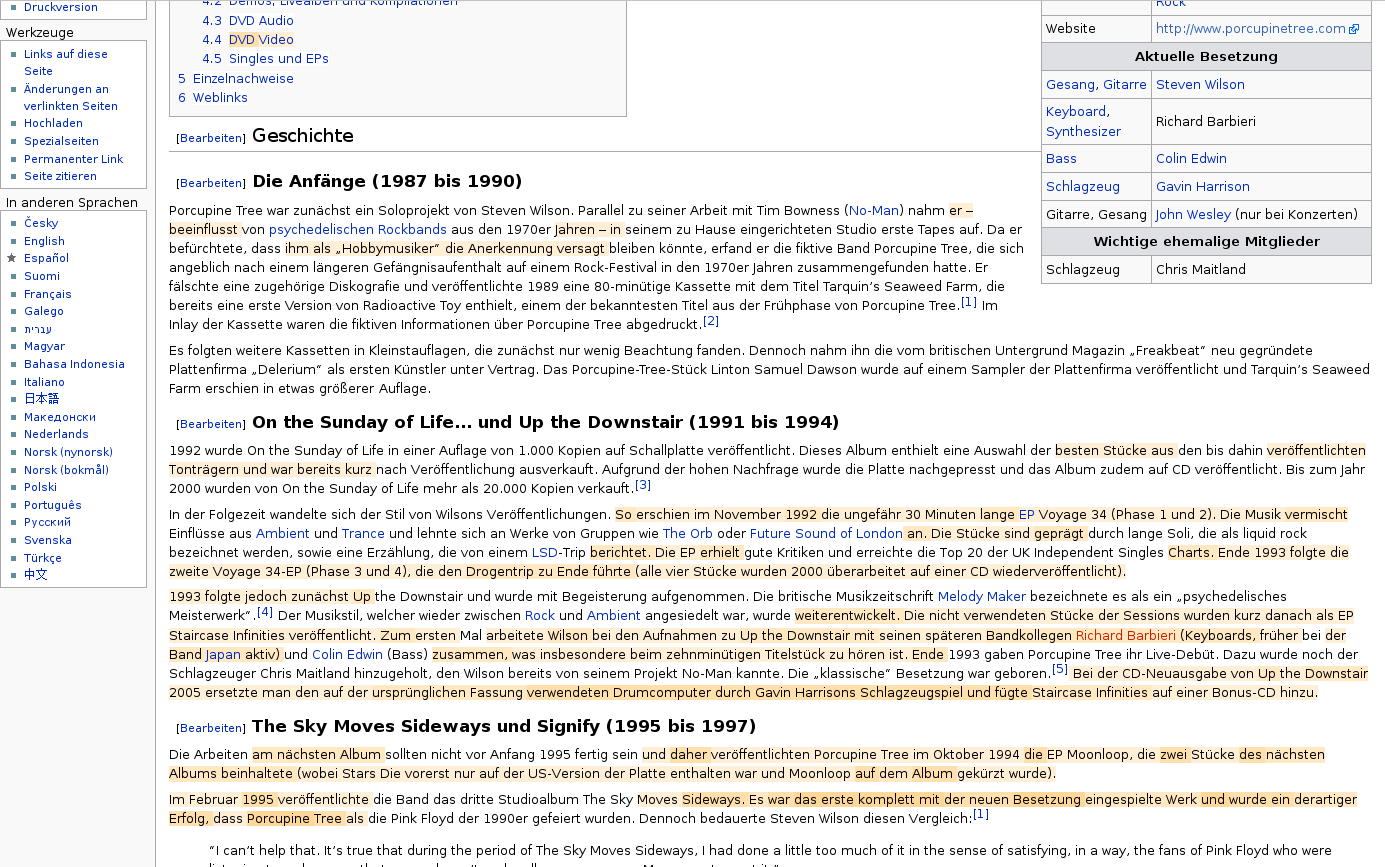
\includegraphics[width=0.8\textwidth,clip=true,resolution=300]{img/wikitrust.png}
  \caption{Wikitrust in action, 2011}
  \label{fig:wikitrust}
\end{figure}

A few other studies present us with useful analyses of edit
behaviour. These studies turn to Wikipedia in order to study user
network interaction, and these analyses of conflict between editors
show the possible reversion cases we will have to automatically
recognise. 

They reveal the high number of immediate `undo'-type revisions, and
also that malicious or unnecessary input may survive several versions
before being undone. Some study these conflicts as a characterisation
of normal editing
behaviour,\cite{Kittur2007}\cite{Kittur2009}\cite{Kittur2010}\cite{Potthast2008}
while others look to controversial articles,\cite{Iba2010} or articles
recently cited in the press.\cite{Lih2004} We find from these same
studies that articles lead by small groups of `leaders' produce
articles of better quality than those with a more homogeneous
contribution group, that a small group of editors contribute to most
of Wikipedia, and that conflict and bureaucracy (increasing over time)
are the major limiting factors in the growth of an
article.\cite{Suh2009} 


% body of thesis comes here

\chapter{Our approach}
\section{Evaluation of methods}
Our methods 

EVALUATE METHODS YO \label{split-distance-eval}

We may consider other ways of looking at the data we have
computed. The gradient factor that we calculate describes how much a
given revision changes in terms of the final state -- it is a real
number from 0 to 1, 0 being a `perfect' move away from the final
version, 1 being a `perfect' move towards. On the trajectory graphs
discussed these two values are represented by a vertical line between
two points, going upwards and downwards, respectively. 

We consider that we could perhaps use it to characterise a 'perfect
edit' -- one that approaches the final edit most efficiently; in a
linear fashion. An optimum revision history may be considered as a
straight path from origin to destination. No edit inserted text that
was later removed, and the approach to the final version was as
efficient as possible over time. We may characterise such an optimum
gradient as follows:


\[
  gfactor_{optimum} = gfactor(ed(rev_{0_{content}},
  rev_{n_{content}}), rev_{n_{tstamp}} - v_{0_{tstamp}})
\]


\textbf{Reversals.} The Damerau-Levenshtein distance defines an `swap'
operation, which is the reversal of two adjacent characters. It is
particularly suited to spell-checking, and for analysing DNA-sequence
variations. In this case:\\ $ed_{damerau}(\text{``ab''},\text{``ba''})
= 1$

\textbf{Block distance.} This allows for displacements of entire
blocks to count as one operation. For
example:\\ $ed_{block}(\text{``abcde''},\text{``cdeax''})= 2$ \\ One
move of the block `cde', one substitution of `b' for
`x'.\cite{Tichy1984}

\subsection*{Density of edit}

If we have a set of the indexes of an edit operation as
$\{op_0,op_1,op_2,\dots, op_n\}$, where $op_i$ is the index of the
$i$th operation, then we may evaluate it's density with a standard
deviation of the edit itself, $\sigma_{ed}$, multiplied by the span of
the edit itself in context of the wider article, and some weighting
factor k. Something along the lines of:
$$ed_{density} = k\bullet\frac{(op_n - op_0)\sigma_{ed}}{|v_{ed}|}$$
where $|v_{ed}|$ is the overall length of resultant version. By
implementing this carefully, we may achieve a gradient of weighting,
with a lower weight values for things like spell-checks, and higher
values for whole-paragraph changes.

\textbf{\textit{q}-grams distance.} \textit{q}-grams are simply
sub-strings, and this measure describes the similarity of two strings
in terms of \textit{q}-grams they
share.\cite{Ukkonen1992}\\ $ed_{q-gram}(x,y)=\sum\limits_{v\in\Sigma
  ^q}|G(x)[v]-G(y)[v]|$\\ where $G(x)[v]$ returns the number of
occurrences of \textit{q}-gram v in string x, and $\Sigma ^q$ is all
the possible \textit{q}-grams in the alphabet (capped by string
length). $|G(x)[v]-G(y)[v]|$ a large positive number every time a
\textit{q}-gram appears a large amount of times in one string, but not
the other; it returns 0 if the substring apears the same number of
times. So, the whole function measures this difference for all
possible substrings, and sums them, returning a high number for
difference, and a low number for similarity.


Other algorithms we may look at are those that, like the
\textit{q}-gram distance, principally concern themselves with finding
common subsequences between the strings. The common subsequence
problem relates to the editdistance problem by way of the
heuristic that two similar strings will have similar subsequences ---
the \textit{q}-gram algorithm, for instance, relies on this heuristic,
and works well for most texts, it does not agree with all distance
measures. For example, two strings that are very different according
to this heuristic may be quite similar according to the
Damrau-Levenshtein measure.


\subsection*{Delta encoding}
Finally, we may also look into Delta encoding algorithms. These
describe ways of compressing the storage of a document's history --- a
format in which only the differences between each text is stored, not
the entire version. These algorithms are of the same family of
algorithms discussed above. In fact, we find that one of the fastest
known algorithms,\footnote{According to Hunt's 1998
  study\cite{Hunt1998}} \textit{VDelta}, is a refinement of the block
distance algorithm mentioned above. For a given version $n$ of a
document $doc$ is defined as:

$$v_n = v_0 \cup {\Delta}(v_0,v_1) \cup {\Delta}(v_1,v_2) \cup \dots
\cup {\Delta}(v_{n-1},v_n) $$

where ${\Delta}(v_i,v_j)$ is the difference between version $i$ and
version $j$ of the document, and the union operation $\cup$ combines
each version in a manner particular to the $\Delta$ data-type. Storing
data in this way can be very efficient, resulting in a compression
factors of five or ten on typical data.\cite{Macdonald2000} It may
also be relatively easy to maintain in our case, due to the linear
nature of Wikipedia revision histories.

%%WEIGHTING BY MARKUP
\subsection*{Identifying and splitting by text species}
Using the wikimedia markup system, we may easily identify certain
species of text. They are as follows:
\begin{itemize*}
\item Internal links
\item External links
\item Images
\item Files
\item Musical scores
\item Math-formatted text (similar to Latex math environment)
\item Section headings (of differing levels)
\item `Citation Needed' tags
\item `As of' tags (used for identification of age-sensitive
  information)
\item Block quotes
\item Tables
\end{itemize*}
\clearpage
We then group them logically, as follows:
\begin{description*}
  \item[Equation]\hfill\\
    Math-formatted text
  \item[Source validation]\hfill\\
    Block quotes, Citations, `Citation Needed' tags, `As of' tags
  \item[Links]\hfill\\
    Internal Links, External Links
  \item[Structural]\hfill\\ 
    Section headings, Tables\\
    It was found in 2005 that this, if anything, was the clearest
    difference between Wikipedia and commercial
    encyclopedias,\cite{Giles2005} supporting previous
    conjecture.\cite{Denning2005} The regexes in this group provide a
    simple way of noticing changes that affect structure.
\end{description*}

We may split the string along the boundaries of these markup tags, and
send levenshtein distance calculator sperate strings, as shown in
figure~\ref{fig:split-diff}.

With these text species grouped, we m. By characterising an edit with
a series of different edit difference we also perhaps create the
opportunity to consider some as more valuable than
others.\label{multiprocessing-bit}

The algorithm that was settled upon left the levenshtein calculator
itself naive of text species -- instead we simply split the text up
and calculate levenstein distance separately. We traverse each string
from beginning to end, using simple regex expressions to identify and
extract different kinds of text, and calculating the levenshtein
distance for each separately. This process is detailed in
algorithm~\ref{dist-calc}. 

%%%%% Distance calculation procedure
\begin{algorithm}
  \caption{Revision pair distance calculation}\label{dist-calc}
  \begin{algorithmic}
    \State $regexes \gets $\{
    \Statex \tab`math1': `$<$math$>$((?!$<${\textbackslash}/math$>$).)*$<${\textbackslash}/math$>${\textbackslash}S',
    \Statex \tab`math2': `\{\{math((?!\}\}).)*\}\}',
    \Statex \tab`bquote': `$<$blockquote$>$((?!$<${\textbackslash}/blockquote$>$).)*$<${\textbackslash}/blockquote$>${\textbackslash}S'
    \Statex  \tab...
    \Statex\}\Comment{Regexes that recognise single Wikimarkup tags}
    \State $reggroups \gets $\{\label{dist-calc-groups}
    \Statex  \tab`maths':(regexes[`math1'], regexes[`math2']),
    \Statex  \tab...
    \Statex \}\Comment{Group of regexes by 'species'}
    \State $distances \gets \emptyset$
    \Function{PairDistance}{$str1,str2$}
    \State $strs \gets [str1, str2]$
    \ForAll {$key, reg \in reggroups$}
    \State $comparestr \gets [``", ``"]$
    \For {$i \gets 0,1$}
    \State $matches \gets reg.matches(strs[i])$
    \ForAll {$m \in matches$}
    \State $match, strs[i] \gets $extractsplit($m.start, m.end, strs[i]$)
    \State $comparestr[i] \gets comparestr[i] + match$
    \EndFor
    \EndFor
    \If {length($comparestr[0]$)$ > 0$ OR length($comparestr[1]$)$ > 0$}
    \State $distances[key] \gets LevDist(comparestr[0], comparestr[1])$ \Comment{See algorithm~\ref{lev-dist}}\label{mprocess-spawn}
    \Else
    \State $distances[key] \gets 0$
    \EndIf
    \EndFor
    \State $distances[$`$norm$'$] \gets LevDist(strs[0], strs[1])$
    \Comment{Process the remainder}
    \State return $distances$\label{mprocess-return}
    \EndFunction
  \end{algorithmic}
\end{algorithm}

In practice, this algorithm was much quicker than trying to add an
awareness of text species to the levenshtein calculator itself. We
using regex statements, we can search and split the string relatively
quickly, and use this preprocessing to alleviate the levenshtein
distance calculator of the burden of being aware of the kinds of text
it is dealing with. With this awareness integrated, because
levenshtein distance considers one character at a time, these
operations of flagging and identifying areas of text were inevitably
multiplied many thousands of time in one operation. Instead we were
able to use a fairly simply algorithm for calculating levenshtein
distance, found in algorithm~\ref{lev-dist}.

\def\HS{\hspace{\fontdimen2\font}}\the\fontdimen2\font

\begin{figure}[p]
  \centering

  \begin{tikzpicture}[
      block1/.style={
        text width=3cm, 
        minimum height=2cm,
        align=center,
        anchor=north,
      },
      block2/.style={
        text width=3cm, 
        minimum height=1.5cm,
        align=center,
        anchor=north,
      },
      font=\small
    ]
    \node (a) [block1] {We can use a [[spork]] to eat spaghetti.};

    \node (b) [block1, right=1cm of a]{We can use [[forks]] to eat lovely
      spaghetti.};

    \node (c) [block1,below=1cm of a]{We can use a \hilight{[[spork]]} to eat
      spaghetti.};

    \node (d) [block1,below=1cm of b]{We can use \hilight{[[forks]]} to eat lovely
      spaghetti.};

    \node (e) [block2,below left=1.5cm and 1.5cm of c] {\hilight{[[spork]]}};
    
    \node (f) [block2,right=1cm of e] {We can use a\HS\HS to eat spaghetti.};

    \node (g) [block2,right=1cm of f] {\hilight{[[forks]]}};
    
    \node (h) [block2,right=1cm of g] {We can use\HS\HS to eat lovely spaghetti.};

    \node (i) [block2,below=1cm of e] {\hilight{[[spork]]}}; 
        
    \node (j) [block2,below=1cm of f] {\hilight{[[forks]]}}; 
    
    \node (k) [block2,below =1cm of g] {We can use a\HS\HS to eat
      spaghetti.};

    \node (l) [block2,below =1cm of h] {We can use\HS\HS to eat lovely spaghetti.};

    \node (m) [block2,below= 1cm of i] {$ed_{links} = 3$};

    \node (n) [block2,below =1cm of k] {$ed_{normal} = 9$};

    \draw [->] (a) -- (c);
    \draw [->] (b) -- (d);
    \draw [->] (c) -- (e);
    \draw [->] (c) -- (f);
    \draw [->] (d) -- (g);
    \draw [->] (d) -- (h);
    \draw [->] (e) -- (i);
    \draw [->] (g) -- (j);
    \draw [->] (f) -- (k);
    \draw [->] (h) -- (l);
    \draw [->] (i) -- (m);
    \draw [->] (j) -- (m);
    \draw [->] (k) -- (n);
    \draw [->] (l) -- (n);

  \end{tikzpicture}
  \caption{Diagram identification of link text, splitting text into
    normal and link segments, and performing separate levenshtein
    distance calculations}
\label{fig:split-diff}
\end{figure}

%%%%% Pair comparison algorithm
\begin{algorithm}[p]
\caption{Pair comparison}\label{pair-comp}
  \begin{algorithmic}
    \Procedure{PairComparison}{$revids$}
    \For {$ i \gets 0, $length($revids$)}
    \If{pair distance not already in database}
    \State $str1 \gets $\LineIf{``"}{$i=0$}{database.gettext($revs[i-1]$)}
    \State $str2 \gets $database.gettext($revs[i]$)
    \State $dist \gets $PairDistance($str1, str2$)\Comment{See algorithm~\ref{dist-calc}}
    \State databaseinsert.pairdistanceinsert($dist$)  
    \EndIf
    \EndFor
  \EndProcedure
  \end{algorithmic}
\end{algorithm}

We will discuss different levenshtein-related algorithms further on
this thesis, but for now we can say that the one we reference here is
fairly basic, but with an optimised space efficiency. We see that we
don't hold a whole matrix for the two strings, only the current and
previous row. We may also describe the PairDistance overall as a
divide-and-conquer algorithm. It improves the space complexity of the
algorithm a little, and allows us the employ parallel or threaded
processing in order to improve efficiency of computation.

\begin{algorithm}
  \begin{algorithmic}
    \Function{LevDist}{$str1, str2$}
    \State $s1len \gets $length($str1$)
    \State $s2len \gets $length($str2$)
    \State $column \gets [0_{1}, 0_{2}, \ldots, 0_{s1len}]$
    \For{$x \gets 1,s2len$}
    \State $col[x] \gets x$
    \EndFor
    \For{$p \gets 1,s1len$}
    \State $column[0] \gets p$
    \State $r \gets p-1$
    \For{$q \gets 1,s2len$}
    \State $oldnum \gets column[q]$
    \State $column[q] \gets min(col[q]+1, col[q-1] + 1, r + str1[p-1] \neq str2[q-1])$
    \EndFor
    \EndFor
    \State return $col[s1len]$
    \EndFunction
  \end{algorithmic}
  \caption{Levenshtein distance calculator}
  \label{lev-dist}
\end{algorithm}

Our procedure for collecting these values is described in
algorithm~\ref{traj-calc}.

%%%%% Trace trajectory algorithm
\begin{algorithm}
  \caption{Page trajectory calculation}
  \label{traj-calc}
  \begin{algorithmic}
    \Procedure{TrajectoryCalculation}{$revids, domain$}
    \State $target \gets $database.gettext($revids[-1]$)\Comment{Last revision in list is most recent}
    \For {$i \gets length(revids), 0$}
    \If{trajectory distance not already in database}
    \State $str1 \gets $database.gettext($revids[i]$)
    \State $dist \gets $LevDist($str1, target$)\Comment{See algorithm~\ref{lev-dist}}
    \State $database.inserttrajectoryinsert(dist)$    
    \EndIf
    \EndFor
    \For{$i \gets 0, length(revids)$}
    \State $dist2 \gets $database.gettrajectory($revids[i],domain$)
    \State $dist1 \gets$
        \LineIf{database.gettrajectory($revid[i-1],domain$)}{$i \neq 0$}{$2 \times disty$}
    \State $time2 \gets $database.gettimestamp($revid[i],domain$)
    \State $time1 \gets $
        \LineIf{database.gettimestamp($revid[i-1],domain$)}{$i \neq 0$}{$timex$} 
    \State ${\Delta}x \gets time2 - time1$
    \State ${\Delta}y \gets dist2 - dist1$
    \If{${\Delta}x > 0$}
    \State $gradient = \frac{arctan({\Delta}y/{\Delta}x)}{\pi}$ 
    \ElsIf{$x = 0$}
    \State $gradient = $\LineIf{1}{$y < 0$}{0}
    \EndIf
    \State database.insertgradient($revid[i],domain,gradient$)
    \EndFor
    \EndProcedure
  \end{algorithmic}
\end{algorithm}

\section{Technology}
Out first stop was to implement a library for tracing a Wikipedia
history, harnessing the Wikipedia API in order to download information
about articles and their histories, as well as their content. It is
inspired by open Wikipedia metadata classes such as `Wikipedia
Miner'\cite{wiki-miner}, or the revision-fetching `Java Wikipedia
Library / Wikipedia Revision
Library'.\cite{wiki-java}\cite{Ferschke2011} The python package
`wikipedia',\cite{python-wikipedia} was also a useful starting point,
but was not appropriate for the project in general.

The Levenshtein distance calcalator, being an intensive computation,
is implemented in C++ for speed purposes. In order to import to
Python, we prepare python variables within the C++ code, and compile
and build a shared object library as defined in the Python
documentation.\cite{python-extend-c++} To further improve speed, we
deploy each levenshtein distance calculation in its own process, to
allow for parallel processing on multi-core machines.

The database is implemented in PostgreSQL, with a python wrapper
written using the psycopg2 module.\cite{psycopg2} The text is
automatically compressed on insertion -- this is the default in
PostreSQL.\cite{psql-comp} 

The graphs are outputted using the matlab-inspired python package,
matplotlib.\cite{matplotlib} 


\chapter{Implementation}
\label{ch:implementation}
\input{implementation/algorithms}


\def \mheight {1cm}
\def \mwidth {2cm}
\definecolor{col2}{HTML}{C7BA9B}
\definecolor{col1}{HTML}{8B7C6D}
\definecolor{col3}{HTML}{F0EAB3}
\definecolor{col4}{HTML}{626072}
\definecolor{col5}{HTML}{40415B}

\tikzstyle{bx}=[
  fill, 
  minimum height=\mheight, 
  minimum width=\mwidth, 
  shape border rotate=90, 
  shape aspect=0.1,
  rounded corners=2mm
]

\tikzstyle{cld}=[
  cloud, 
  cloud puffs=15.7, 
  cloud ignores aspect, 
  minimum height=\mheight,
  minimum width=\mwidth, 
  align=center
]

\tikzstyle{dtb}=[
  fill,
  chamfered rectangle,
  chamfered rectangle xsep=2cm,
  minimum height=\mheight, 
  minimum width=\mwidth,
  rounded corners=1mm
]

%% \tikzstyle{box}[draw,minimum height=5em,minimum width=10em]

\begin{figure}
  \centering
  \begin{tikzpicture}[align=center,node distance=2cm]

    \node (database)[dtb, fill=col1]{Database};

    \node (wikidata)[bx, fill=col2, above=of database]{WikiDatabase};

    \node (analysis)[bx, fill=col2, above=of wikidata]{WikiAnalysis};

    \node (wikifetch)[bx, fill=col2, left=0.5\mwidth of analysis]{WikiRevisionScrape};

    \node (datahandle)[bx, fill=col2, right=0.5\mwidth of analysis]{WikiDataHandle};
    
    \node (intplot)[bx, fill=col2, above of=datahandle]{WikiInteractivePlot};
    
    \node (datplot)[bx, fill=col2,  right=0.5\mwidth of intplot]{WikiDataPlot};

    \node (wikicli)[bx, fill=col5, above= 3cm of analysis]{WikiCLI}; 
    
    \node (wikipedia)[cld, fill=col4, left=of wikicli]{\textit{Wikipedia
        API}};

    \draw [-] (database) -- (wikidata); 

    \draw [-] (wikidata) -- (analysis); 

    \draw [-] (wikidata) -- (wikifetch); 

    \draw [-] (wikidata) -- (datahandle); 

    \draw [-] (wikifetch) -- (wikipedia); 

    \draw [-] (datahandle) -- (intplot); 

    \draw [-] (datahandle) -- (datplot);

    \draw [-] (intplot) -- (wikicli); 

    \draw [-] (datplot.north) -- (wikicli); 

    \draw [-] (wikifetch) -- (wikicli); 

    \draw [-] (wikicli) -- (analysis); 

    \node (blob) [
      draw=col5, 
      fit= (wikidata) (datplot) (wikifetch), 
      inner sep=0.4cm,
      thick,
      rounded corners=8mm
    ] {};

    \node [
      col5, 
      anchor=south east, 
      xshift=-4mm,
      yshift=4mm
    ] at (blob.south east) {\textbf{the WikiRevision package}};

  \end{tikzpicture}

  \caption{Diagram showing the connections between entities in python implementation}
\end{figure}

\section{Guide to the code}
Appendix

The project was implemented in Python, with a C++ core for the
Levenshtein distance implementation. The code runs reasonably quikly,
with it's speed mainly limited by the speed of the HTTP requests, and
the speed of the database. To compute Levenshtein distance we employ a
short C++ script that returns Python-variables, and is compiled into a
shared object library for use in Python. 

Here we discuss the five main classes in the project, and their
function in this project.

\subsection*{WikiData}
The wikidata module interfaces with the database, and maintains its
integrity. 

\subsection*{DataHandle}
In this class we find the functions that prepare the data in the
database for plotting, including weighting results if necessary. From
the CLI. 

\subsection*{WikiDataPlot}
Data Plot can be run as a script, or instantiated as a class and run
manually. Running as a script automatically runs the DumpPlot
function, picking random pages from the database to plot, as well as
reporting various metrics regarding the revisions that are currently
stored in the database. The figures used in the discussion of results
section are procduced by this function. Otherwise, the lineGraph,
barChart and trajectoryGraph functions are self-explanatory. These
files will be output from the CLI given the \textit{-p} option.

The IPlot function runs a simple PyQT widget, showing results regarding a
particular page (or a random page if unspecified). It can be run from
the CLI using the \textit{-i} argument.

\subsection*{WikiFetch}
Contains implementation of algorithm REFERENCE, including all the
necessary logical extensions to deal with CLI parameters such as the
'depth' argument, etc. It interfaces with various Wikipedia websites. 

It holds a file, scraped from the English Wikipedia, of the various
existing Wikipedia sub-domains (English (en.), German (de.), Italian
(it.), etc.), and picks it's domain name from that if asked to. This
class is engaged by the CLI.

\subsection*{WikiAnalysis}
An implementation of the algorithm found at REFERENCE. We employ
threading to speed the computation up on multi-core systems, computing
levenshtein each separate species of text in a separate thread, as
shown in figure~\ref{fig:threading}. Although (as shown in figure
FIGURE) we expect that the 'normal' text portion comparison is
inevitably longer than any non-normal, and we execute this thread last
(being the remainder text), so we would expect to be waiting on this
thread before the computation exits. Never-the-less, we found a
notable increase in performance by implementing threading.

We may extend this by allowing for that final `normal' text to be
split down into different strings, and computed in separate threads on
separate cores. We use a 'core number' variable to that end.

\begin{figure}
  \centering
  \begin{tikzpicture}[x=0.5cm, y=0.5cm]
    \draw[step=.1cm,gray,very thin] (0,6) grid (30,5);
    \draw[step=.1cm,gray,very thin] (0,4) grid (30,3);
    \draw[step=.1cm,gray,very thin] (0,2) grid (30,1);
    \draw(0,0) rectangle (30,-1);
  \end{tikzpicture}
  \caption{Diagram showing multi-processing in pair distance calculation}
\end{figure}

\subsection*{The Database}
The database is implemented in PSQL, and accessed via our python
package, `wikiDatabase'. The package leverages the psycopg library,
which allows simple access to the SQL database via
python.\cite{psycopg2} The package is used by all the other classes
used in this project and provides simple inserting, changing, fetching
and checking of data.

Some more complex operations are undertaken by the class, mainly
preparing large `data-dumps' for mass-plotting (inpreparation for this
report) and validation exercises. These functions were written for
performance purpose (the data they deliver could eaily have been
fetched using the other functions, but would have taken much longer),
and are clearly marked in the code as seperate from the basic fetch,
get and insert functions. 

The database relies upon the uniqueness of revision ID and
domain-name, and page ID and domain-name pairs.  pairs to
function. The existing database schemata can be found in
figure~\ref{database-schema}. We talk about improving this schemata in
the evaluation chapter.

\begin{figure}
  \centering
  \begin{subfigure}[t]{0.3\linewidth}
    \centering
    \begin{tabular}{ccc}
      \toprule
      \underline{revid} & \underline{domain} & content\\
      \midrule
      $\vdots$ & $\vdots$ & $\vdots$\\
    \end{tabular}
    \caption{Table: wikicontent}
  \end{subfigure}
  \begin{subfigure}[t]{0.2\linewidth}
    \centering
    \begin{tabular}{cc}
      \toprule
      \underline{pageid} & \underline{domain} \\
      \midrule
      $\vdots$ & $\vdots$\\
    \end{tabular}
    \caption{Table: wikifetched}
  \end{subfigure}
  \begin{subfigure}[t]{0.4\linewidth}
    \centering
    \begin{tabular}{cccc}
      \toprule
      \underline{revid1} & \underline{revid2} & \underline{domain} & distance\\
      \midrule
      $\vdots$ & $\vdots$ & $\vdots$ & $\vdots$ \\
    \end{tabular}
    \caption{Table: wikitrajectory}
  \end{subfigure}\\
  \vspace{10 mm}
  \begin{subfigure}[b!]{\linewidth}
    \centering
    \begin{tabular}{ccccccccc}
      \toprule
      \underline{revid} & \underline{domain} & pageid & title & username & userid & time & size &
      comment \\ 
      \midrule
      $\vdots$ & $\vdots$ & $\vdots$ & $\vdots$ & $\vdots$ & $\vdots$ & $\vdots$
      & $\vdots$ & $\vdots$ \\
    \end{tabular}
    \caption{Table: wikirevisions}
  \end{subfigure}
  \vspace{30 mm}
  \begin{subfigure}[b!]{\linewidth}
    \centering
    \begin{tabular}{ccccccccc}
      \toprule
      \underline{revid} & \underline{domain} & maths & citations & filesimages & links &
      structure & normal & gradient\\
      \midrule
      $\vdots$ & $\vdots$ & $\vdots$ & $\vdots$ & $\vdots$ & $\vdots$ &
      $\vdots$ & $\vdots$ & $\vdots$ \\
    \end{tabular}
    \caption{Table: wikiweights} 
  \end{subfigure}
  \caption{Schemata for the database used to store wikipedia data}
  \label{database-schema}
\end{figure}

TALK ABOUT schema.sql, dump.sql

\section{The interface}
The CLI can be accessed using the shortcut wrhp (Wiki Revision History
Portal...). The arguments are as follows:

\begin{itemize}[label={}]
  \item \textbf{Default behvaiour.} Default behaviour is -s.
  \item \textbf{-s} Scrape and analyse. Attempts to fetch a new page
    to the database, and process it. If used with -p or -i, means to
    attempt to collect a new page from the site before plotting,
    rather than taking one from the database.
  \item \textbf{-p} Plot data. Saves png files to location given by
    the --plotpath argument.
  \item \textbf{-i} Open the interactive plot window for a given (or
    random) article once analysed.
  \item \textbf{-v} View a Wikipedia page online. Must be used with
    --domain. Can be used to view a diff (using --revid and
    --oldrevid), a specific revision (using only --revid), or the
    latest version of a page (using --pageid).
  \item \textbf{-t} `Trundle' mode. Repeats the given operation until
    interrupted. Useful for building up a database. Cannot be used
    with the --titles argument.
  \item \textbf{--title [\textit{str}]} Specify the
    pages to be scraped. Must be used with --domain. Case (and
    spelling...)  sensitive.
  \item \textbf{--domain [\textit{str}]} Specify the domain to connect
    to. May be used without --titles, limiting the random page pick to
    one domain. Must be the short version (`en', `de', etc.).
  \item \textbf{--scrapemin [\textit{int}]} Specify the minimum amount of
    pages to be scraped for one page. Default = 50.
  \item \textbf{--plotpath [\textit{filepath}]} Specify location for
    plots to be stored. Default = .
  \item \textbf{--revid} Specify the revision ID to be viewed. Used
    with -v.
  \item \textbf{--oldrevid} Specify the old revision ID when viewing a
    diff. Used with -v/
  \item \textbf{--pageid} Specify a target pageid. Can be used in -v
    and -s.
\end{itemize}


\chapter{Results}
\label{ch:results}
\chapter {Discussion}
The following discussion makes reference to included graphs, but also
to online sources, such as wikipedia revision diffs. The 

\section{Results}
The basic output of the model described here is a set of numbers, a
levenshtein distance for each of the groups described in
line~\ref{dist-calc-groups} of algorithm~\ref{dist-calc} (and
described more clearly by the schema in figure~\ref{weightstable}),
and a trajectory factor, calculated by the procedure found in
algorithm~\ref{traj-calc}. As such, the output can be analysed in
numerous ways.

Our basic analysis is based on the following three measures:
\begin{itemize}[]
\item \textbf{Trajectory graph.} This plots the change of the article
  over time. By measuring a levenshtein distance between each revision
  text against the final version (see algorithm~\ref{traj-calc}), we
  see the article in terms of its growth from an empty article, and
  the approach to its final version. We also plot the size of the
  article at each point of this graph for greater context.
\item \textbf{User by share.} We sum up each user's 'share' of the
  article using the calculations made during analysis, and order them
  here by user.
\item \textbf{User by edit count.} Our understanding of the previous
  graph can be made greater if we understand how many edits each user
  has made.
\end{itemize}

\section{Analysis}
\subsection*{Trajectory plots}
We noticed a number of notable things using these plots. But, on
average, they follow a similar pattern: the levnshtein distance of the
article begins at a high value at $x=0$, it's creation date, and
approaches the final article state at $y=0$ and a high value of $x$
(with the final article having a levenshtein distance of $0$ to
itself). In this simplest case, the growth of the article is a rough
mirror-image of the distance-to-final, beginning at the origin and
rising. A few of these `classic' examples can be found in
figure~\ref{fig:traj-classic}.

\begin{figure}
  \label{fig:traj-classic}
  \centering
  \makebox[\linewidth][c]{
    \begin{subfigure}[b!]{0.6\linewidth}
      \centering
      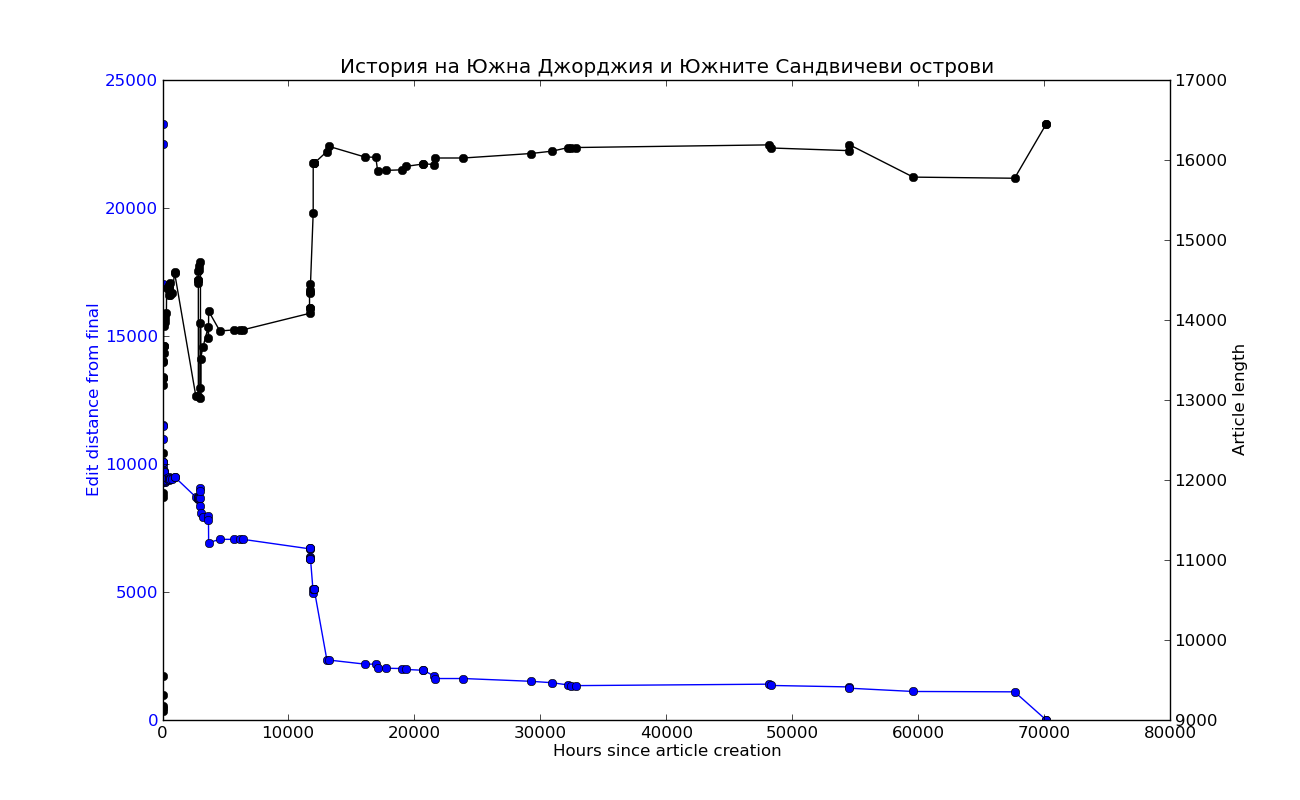
\includegraphics[width=\linewidth]{img/traj-classic/bg90882traj.png}
      \caption{\href{http://bg.wikipedia.org/wiki/index.php?curid=90882}{Bulgarian
      Wikipedia, Page ID 90882 (History of South Georgia and the South Sandwich Islands)}}
    \end{subfigure}
    \begin{subfigure}[b!]{0.6\linewidth}
      \centering
      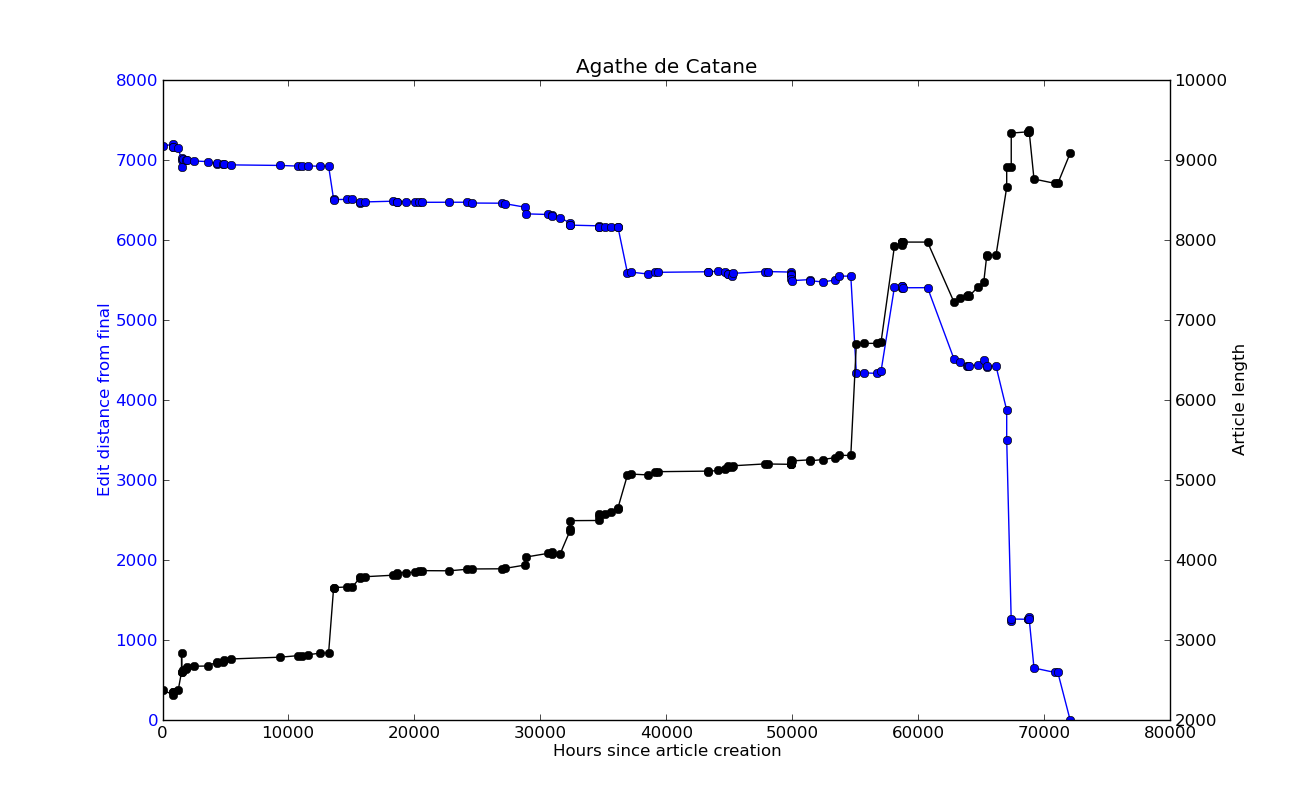
\includegraphics[width=\linewidth]{img/traj-classic/fr572796traj.png}
      \caption{\href{http://fr.wikipedia.org/wiki/index.php?curid=572796}{French
      Wikipedia, Page ID 572796 (Agatha of Catania)}}
    \end{subfigure}
  }\\
  \makebox[\linewidth][c]{
    \begin{subfigure}[b!]{0.6\linewidth}
      \centering
      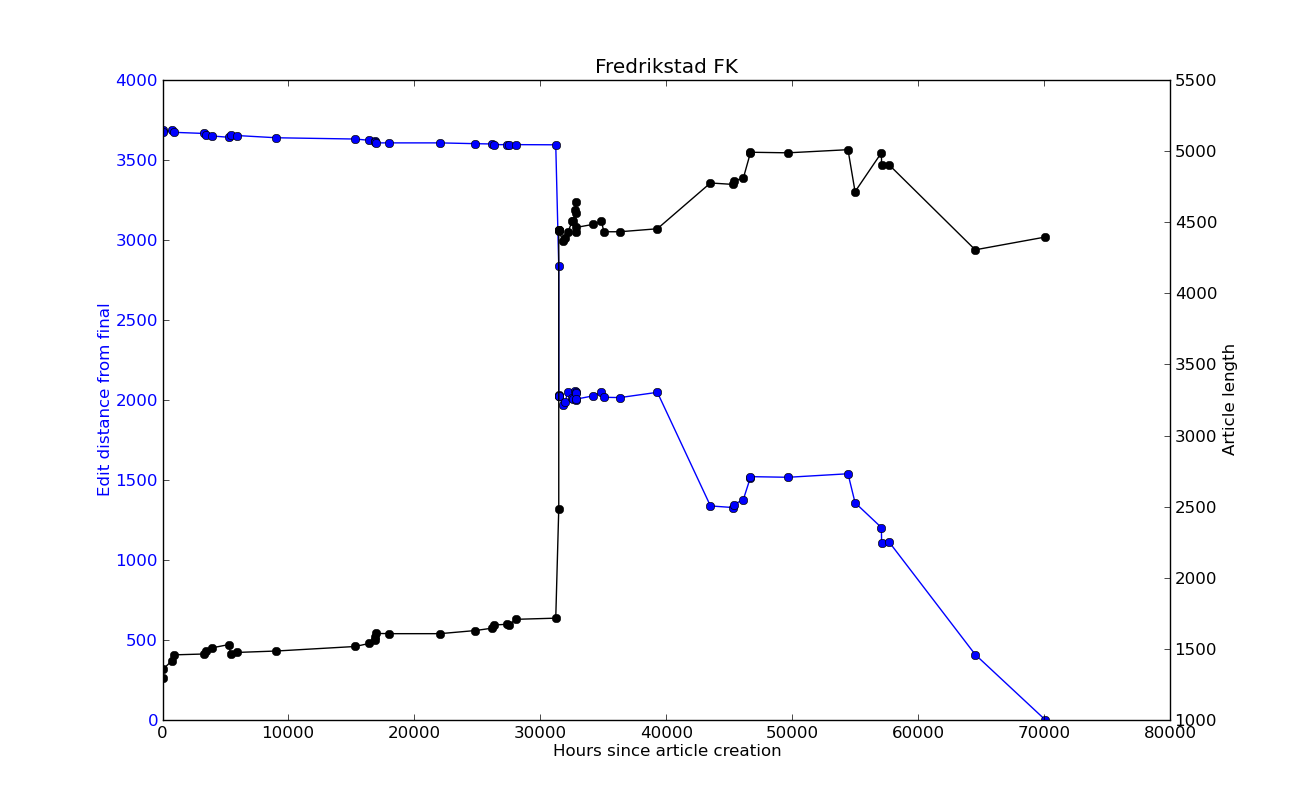
\includegraphics[width=\linewidth]{img/traj-classic/pl291709traj.png}
      \caption{\href{http://pl.wikipedia.org/wiki/index.php?curid=291709}{Polish
      Wikipedia, Page ID 291709 (Fredrikstad FK, a Norwegian football
      club)}}
      \label{fig:fredrikstad}
    \end{subfigure}
    \begin{subfigure}[b!]{0.6\linewidth}
      \centering
      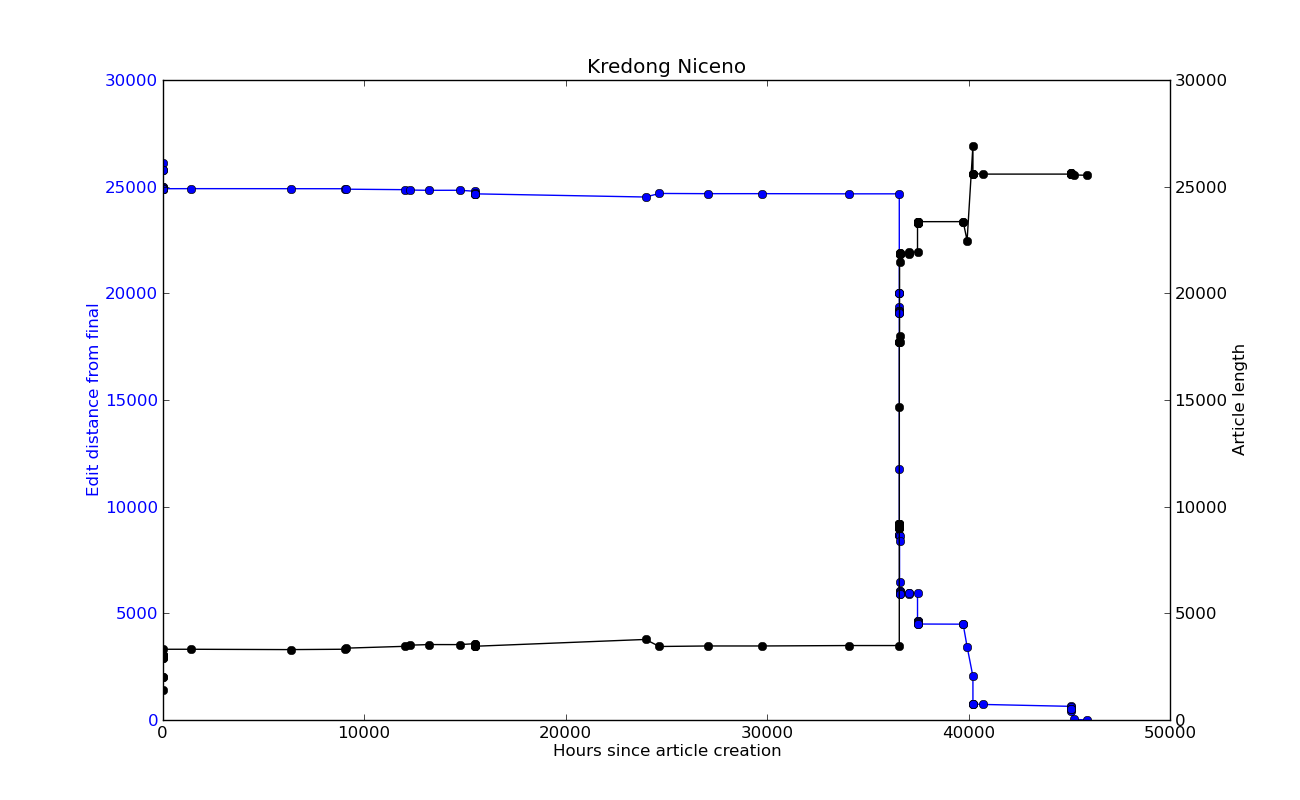
\includegraphics[width=\linewidth]{img/traj-classic/tl62286traj.png}
      \caption{\href{http://tl.wikipedia.org/wiki/index.php?curid=62286}{Tagalog
      Wikipedia, Page ID 62286 (The Nicene Creed)}}
      \label{fig:nicine-creed}
    \end{subfigure}
  }\\
  \makebox[\linewidth][c]{
    \begin{subfigure}[b!]{0.6\linewidth}
      \centering
      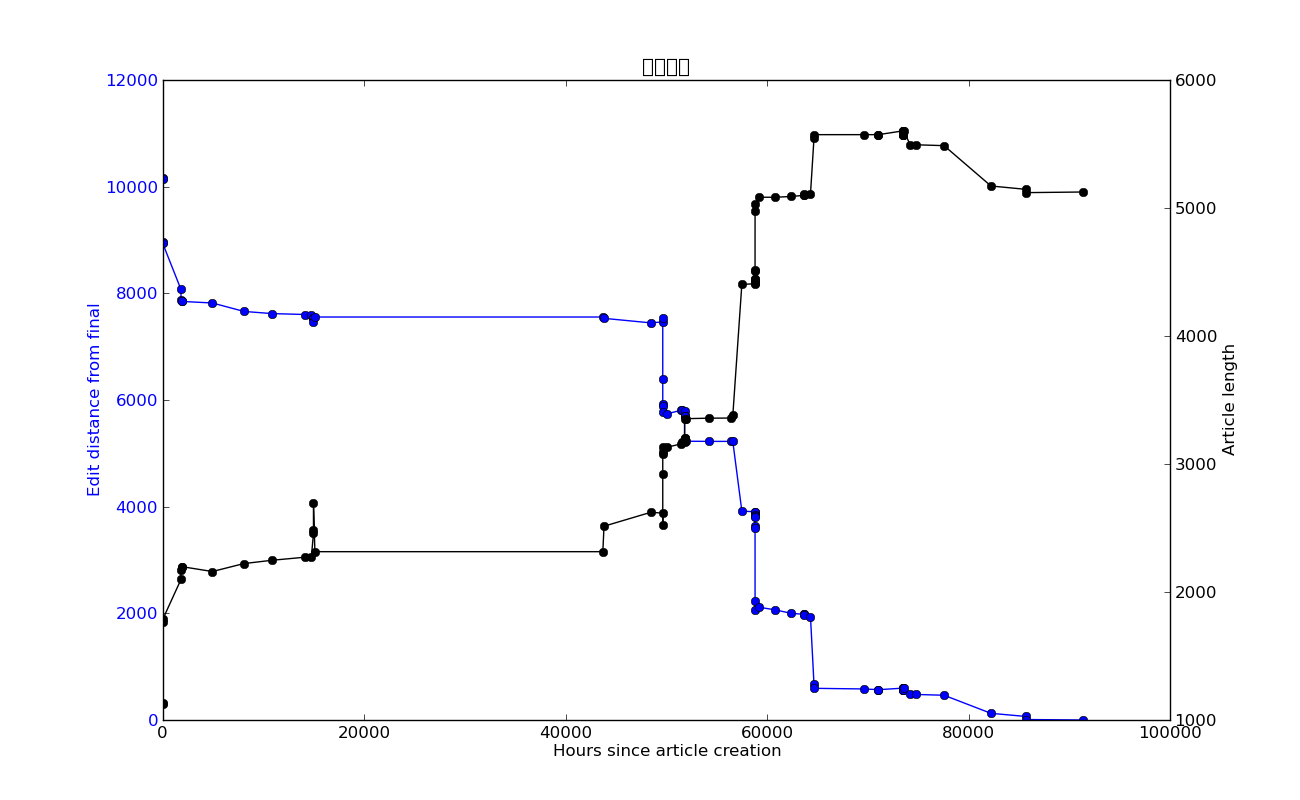
\includegraphics[width=\linewidth]{img/traj-classic/ja1611162traj.png}
      \caption{\href{http://ja.wikipedia.org/wiki/index.php?curid=1611162}{Japanese
      Wikipedia, Page ID 1611162 (The Tax Treaty)}}
      \label{fig:japanese-tax}
    \end{subfigure}
    \begin{subfigure}[b!]{0.6\linewidth}
      \centering
      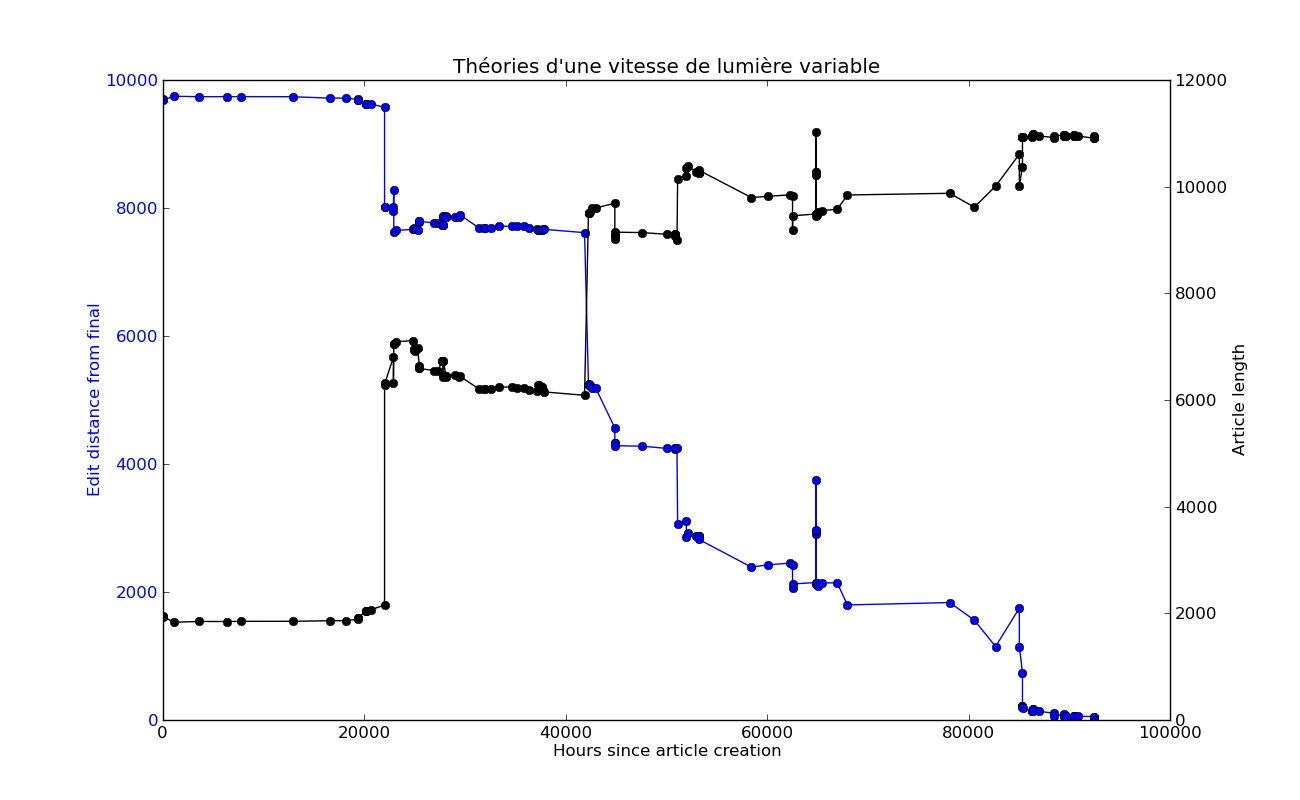
\includegraphics[width=\linewidth]{img/traj-classic/fr43937traj.png}
      \caption{\href{http://fr.wikipedia.org/wiki/index.php?curid=43937}{French
      Wikipedia, Page ID 43937 (Theories of a variable light speed)}}
      \label{fig:variable-light}
    \end{subfigure}
  }
  \caption{Simple trajectory graphs.}
\end{figure}

In the last of these simple trajectory graphs we find the first of our
notable features. Figure~\ref{fig:variable-light} shows a clear sign
of an undo operation at around 65,000 into the age of the article. We
see the black line take a steep ascent and immediate descent, showing
a quick enlargement and reduction of the article size. Since the same
spike can be seen in the blue line, we know that inserting this text
made the the article more different from the final version, and the
removed text brought us back. We can infer that the same text that was
added was the same as that which was removed. We find one of these
redo-undo edits
\href{http://fr.wikipedia.org/w/index.php?title=Th\%C3\%A9ories\_d\%27une\_vitesse\_de\_lumi\%C3\%A8re\_variable&diff=96659084&oldid=96654283}{in
  the wikipedia diff between revids 96659084 and 96654283}.

In contrast, the Phillipino article on the Nicene Creed
(Figure~\ref{fig:nicene-creed}) has a similar-shaped spike in it's
size. The event can be seen to occur just after 40000 hours. In this
case however, the trajectory line does not spike in turn. In this case
we can assume that the inserted spike shows an insertion of text that
remains in the article, and the deletion of text that is not
re-inserted before the article's current version.

These spikes are fairly obvious characteristics to identify on plots
such as these. However, we may also identify longer periods of
meandering away from and back towards the current version. Notice the
arced paths in figure~\ref{fig:fredrikstad}, spanning around 45000 to
55000 hours. Although the time frame is much larger than in the other
articles (10,000 hours $\approx$ 1 year 2 months), and multiple edits
occur in the meantime, we may also characterise the overall event as
an `undo' operation. It is more nuanced than others we have identified
so far (after the event the article is equally similar to the current
version, but smaller in size), but the effect is the same. The burden
is upon our model as to how to sufficiently characterise these
long-term discardations of useless inserted material.

We also may begin to notice that that edits may tend to cluster in
time, and that the articles may owe much of their content one-time
bursts of activity. The Japanese article on tax
(figure~\ref{fig:japanese-tax}), after an `undo'-shaped cluster of
edits at around 15000 hours, was not edited again for almost 3
years. The Tagalog and Polish articles (respectively the smallest and
largest articles discussed so far) gained most their content over just
a few days. 

However, many of the trajectories we trace bely a much stranger
history. Those in figure~\ref{fig:traj-bot} show a particular feature
a slow climb in both distance-from-final and size, before a sharp
drop. The shape is very common, and seems to describe an article which
becomes slowly bigger, before having the majority of it's content
deleted. In plotting the histories it seemed to occur very often, and
on further inspection we find each article to share two
characteristics -- they come from small Wikipedias, and the majority
of the edits are made by bots.\footnote{We can see from the usernames on the
right-hand side graphs in figure~\ref{fig:traj-bot} that they are bots
-- there is a special bot `flag' to be raised in the user profile of
bots, but it is also traditional for the bot to be also be given an
identifying name.\cite{wiki-bot-policy}}
 
\begin{figure}
  \label{fig:traj-bot}
  \centering
  \makebox[\linewidth][c]{
    \begin{subfigure}[b!]{1.2\linewidth}
      \centering
      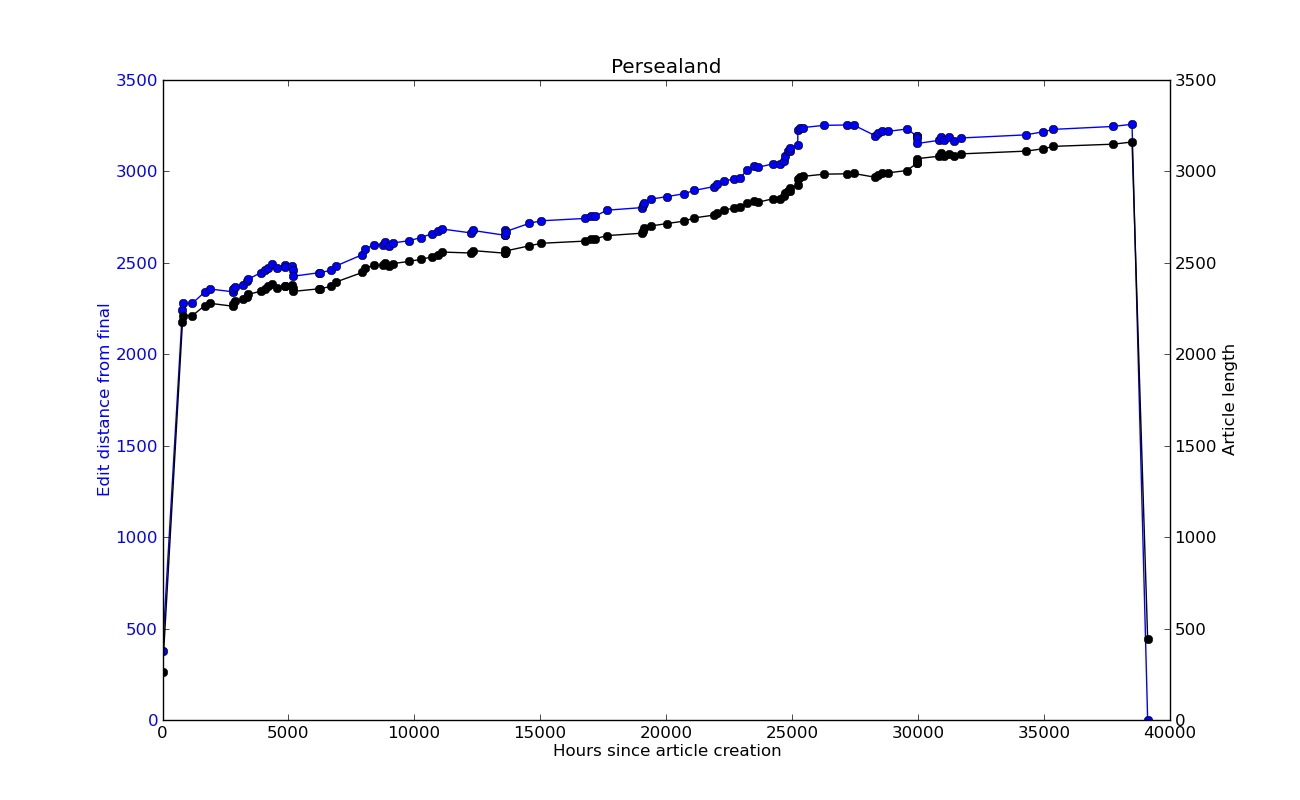
\includegraphics[width=0.45\linewidth]{img/traj-bot/ang7120traj.png}
      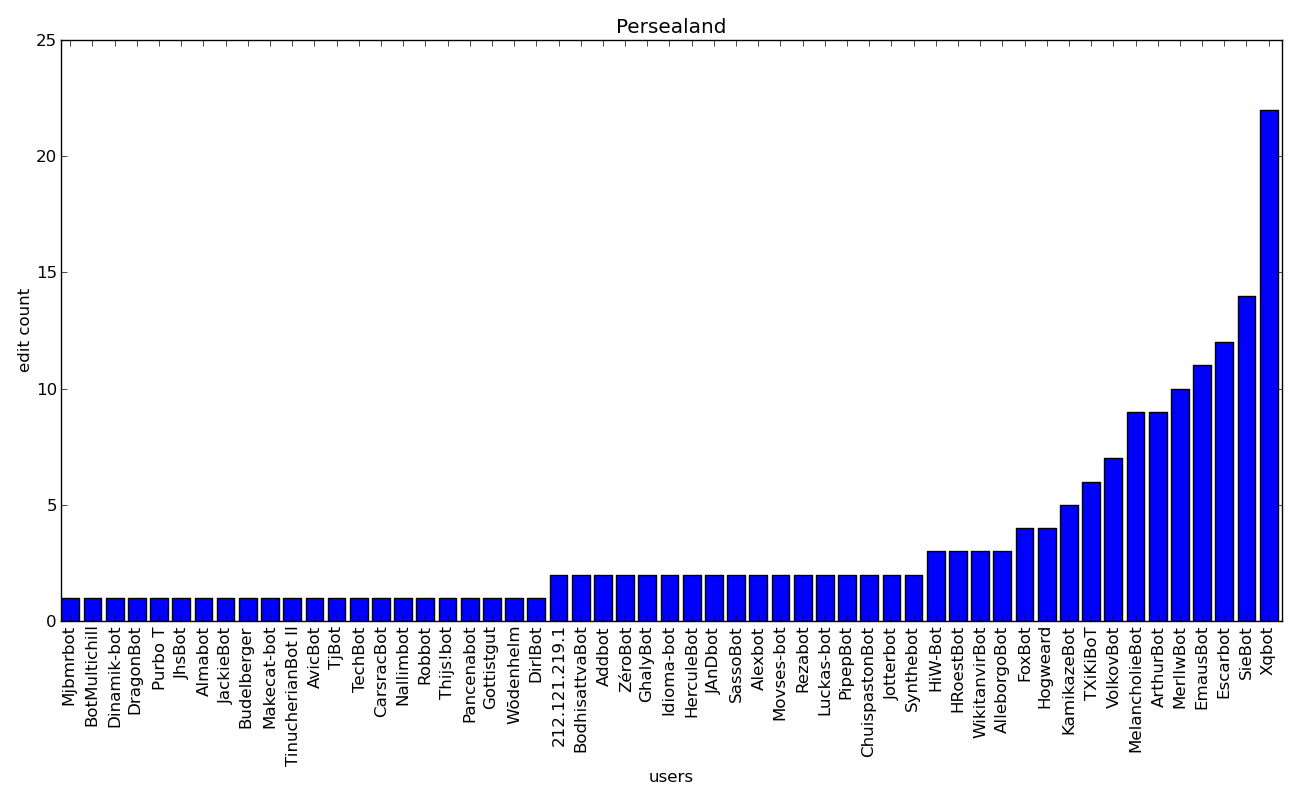
\includegraphics[width=0.45\linewidth]{img/traj-bot/ang7120users.png}
      \caption{\href{http://ang.wikipedia.org/wiki/index.php?curid=7120}{Anglo-Saxon
      Wikipedia, Page ID 7120 (Persia)}}
    \end{subfigure}
  }\\
  \makebox[\linewidth][c]{
    \begin{subfigure}[b!]{1.2\linewidth}
      \centering
      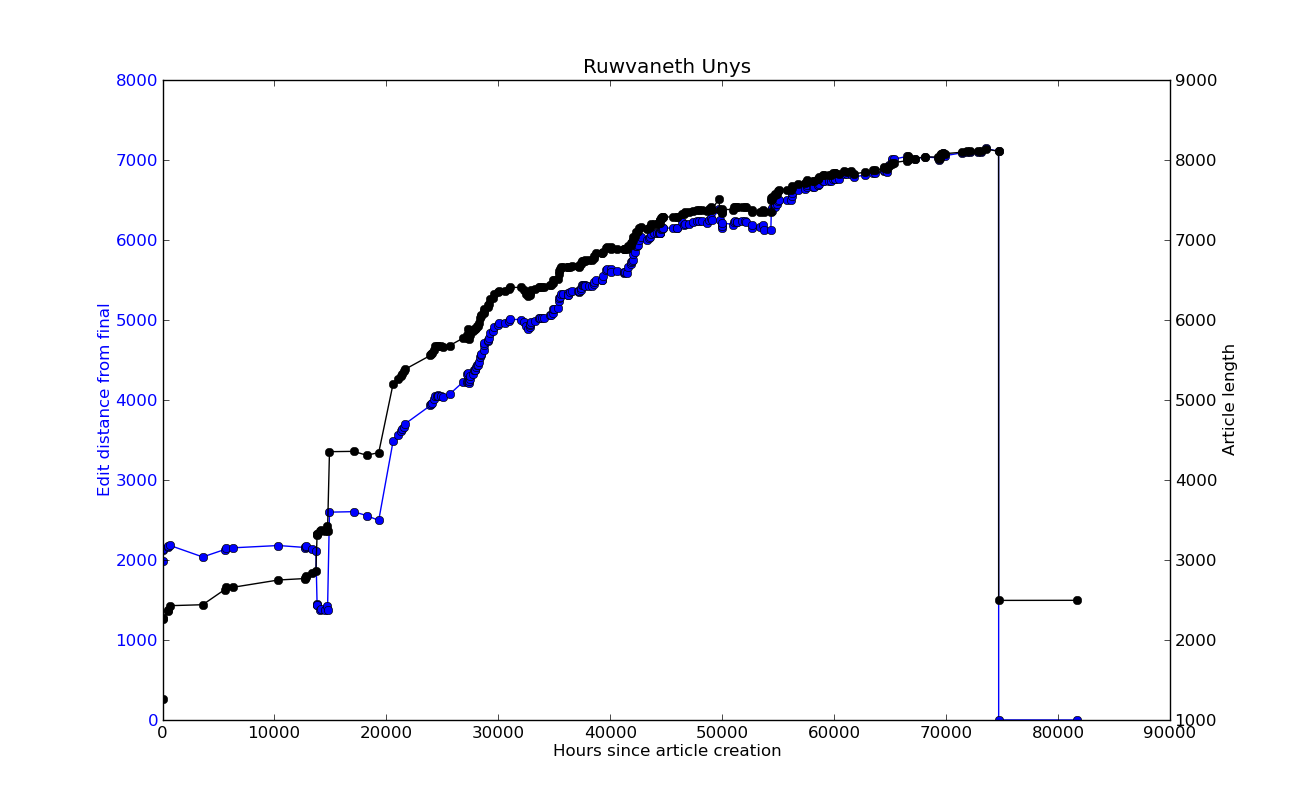
\includegraphics[width=0.45\linewidth]{img/traj-bot/kw736traj.png}
      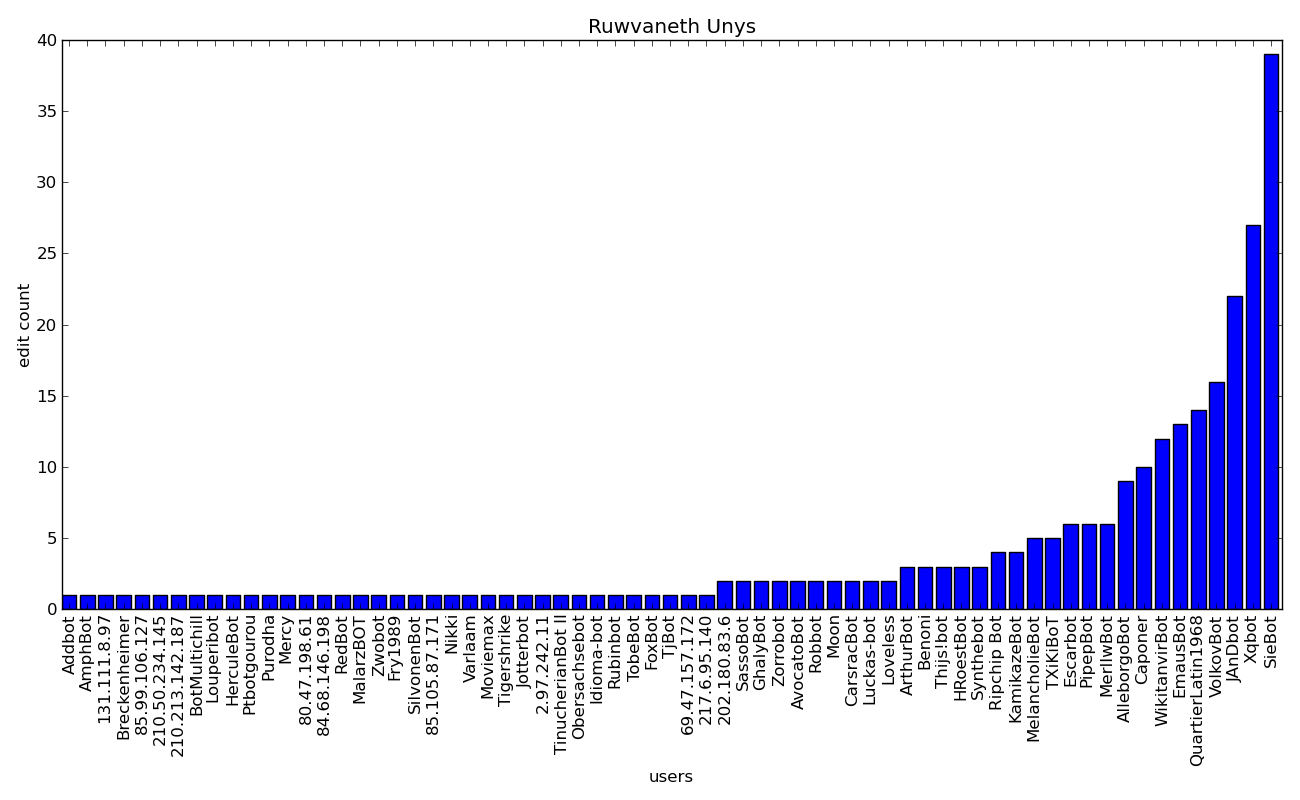
\includegraphics[width=0.45\linewidth]{img/traj-bot/kw736users.png}
      \caption{\href{http://kw.wikipedia.org/wiki/index.php?curid=736}{Cornish
      Wikipedia, Page ID 726 (United Kingdom)}}
    \end{subfigure}
  }\\
  \makebox[\linewidth][c]{
    \begin{subfigure}[b!]{1.2\linewidth}
      \centering
      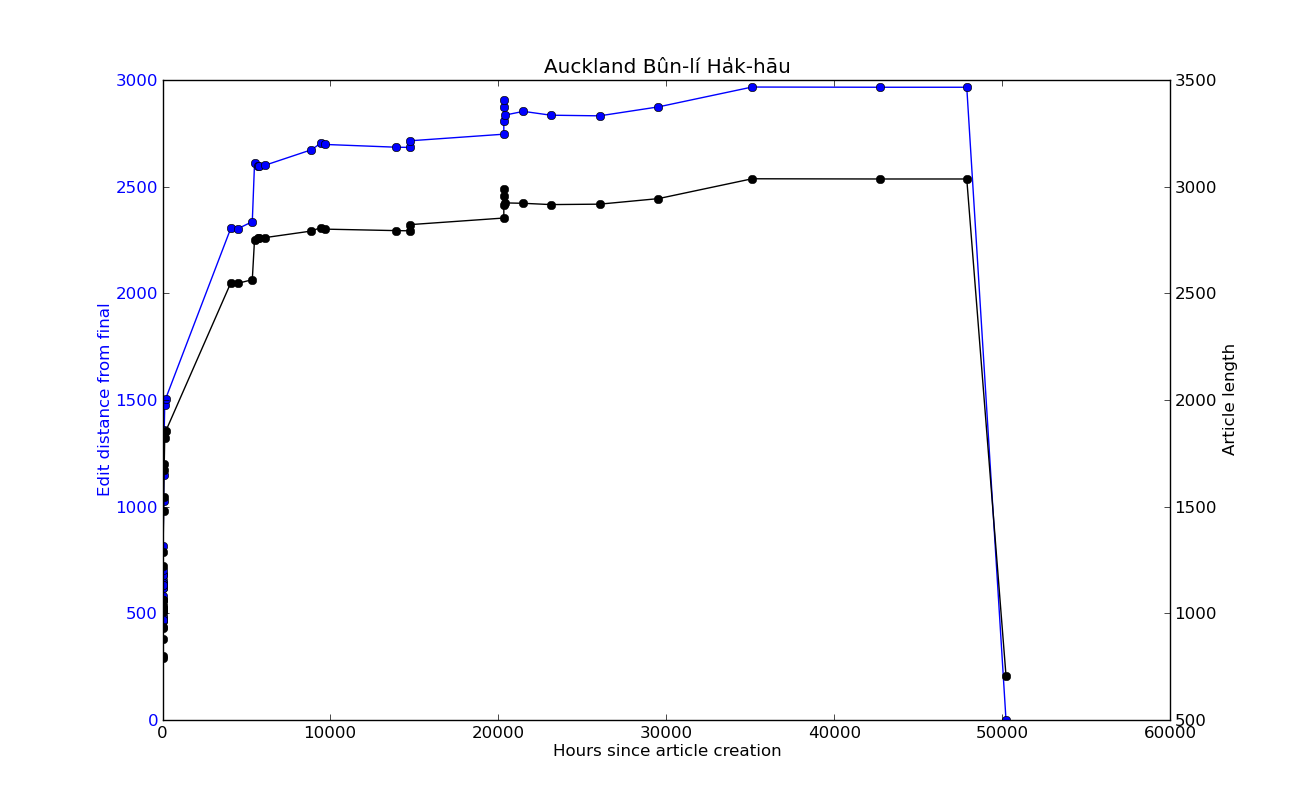
\includegraphics[width=0.45\linewidth]{img/traj-bot/zh-min-nan10733traj.png}
      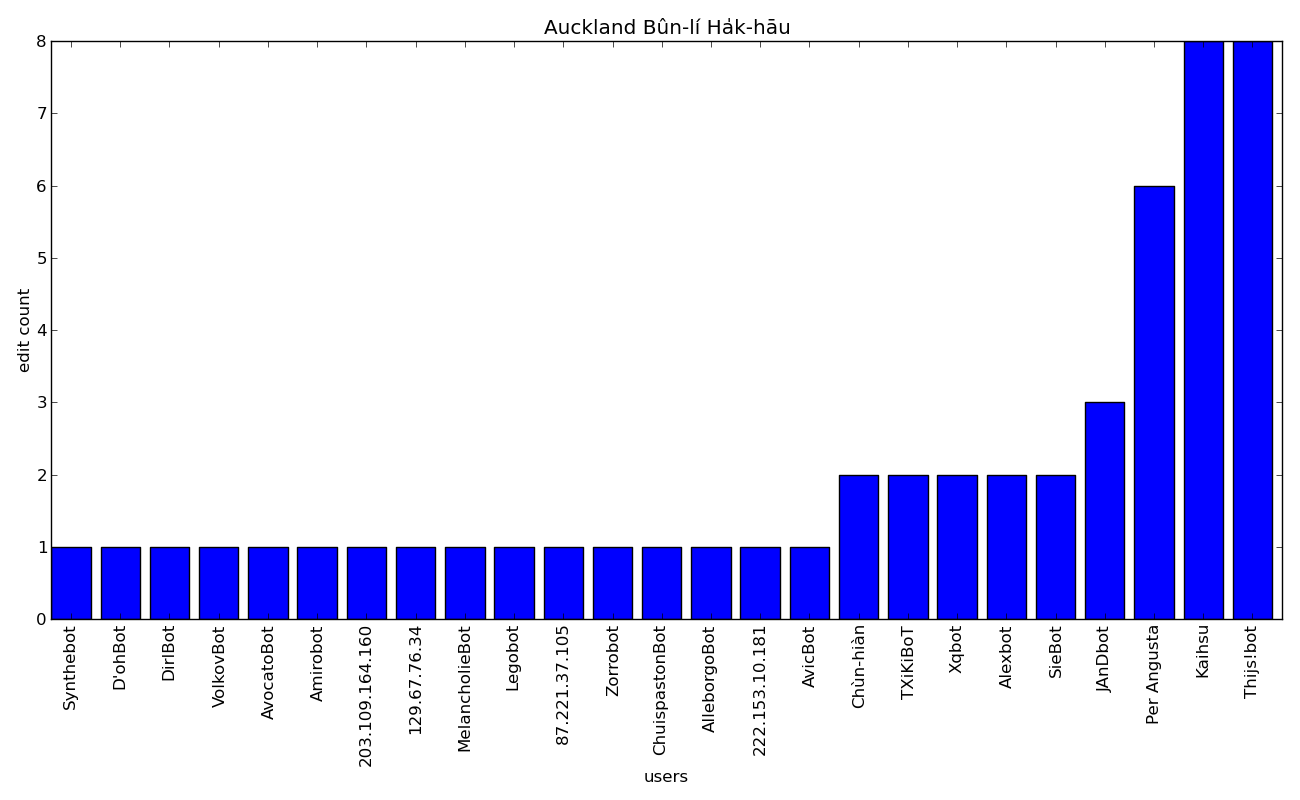
\includegraphics[width=0.45\linewidth]{img/traj-bot/zh-min-nan10733users.png}
      \caption{\href{http://zh-min-nan.wikipedia.org/wiki/index.php?curid=10733}{Min Nan
      Wikipedia, Page ID 10733 (Auckland Grammar School)}}
    \end{subfigure}
  }\\
\caption{Trajectory graphs showing bot editing characteristics.}
\end{figure}

The explanation is in the articles' histories. In each one, we find a
single large deletion event, ocurring any time after early 2013. With
a little digging, we find the origin of the act to be a Wikimedia
project that aims to `migrating interlanguage wiki links from
individual articles into a central database to ease
maintenance',\cite{wiki-interwikilinks} see
figure~\ref{traj-bot-explanation} for evidence of just one of these
events. Each wikipedia article is rendered to the right of a language
bar that links that article to its counterpart in various
languages. Once coded into each article manually, that data is now
stored in and served from a central source.\cite{wiki-blog-onwikidata}
The move gives us strange results for this project -- for small
articles, the loss of these hard-coded links constitutes a gutting of
its majority content. By our measurements, in these circumstances,
this act of housekeeping is a momentous event in the history of small
articles.

\begin{figure}
  \label{fig:traj-bot-explanation}
  \centering
  \makebox[\linewidth][c]{
    \begin{subfigure}[b!]{1.2\linewidth}
      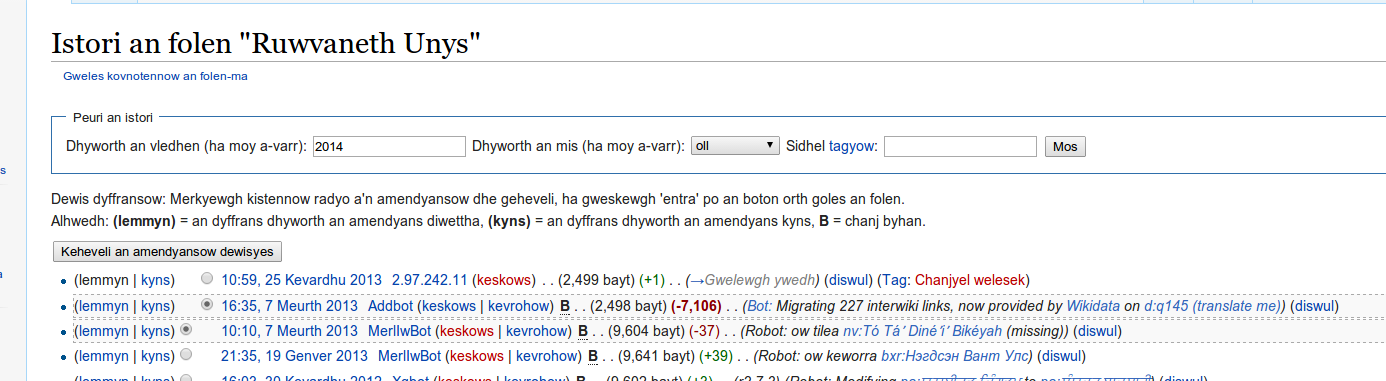
\includegraphics[width=1\linewidth]{img/traj-bot/botmigration.png}
      \caption{Migration event in article history (16:35, 7 March 2013)}
    \end{subfigure}
  }\\
  \makebox[\linewidth][c]{
    \begin{subfigure}[b!]{1.2\linewidth}
      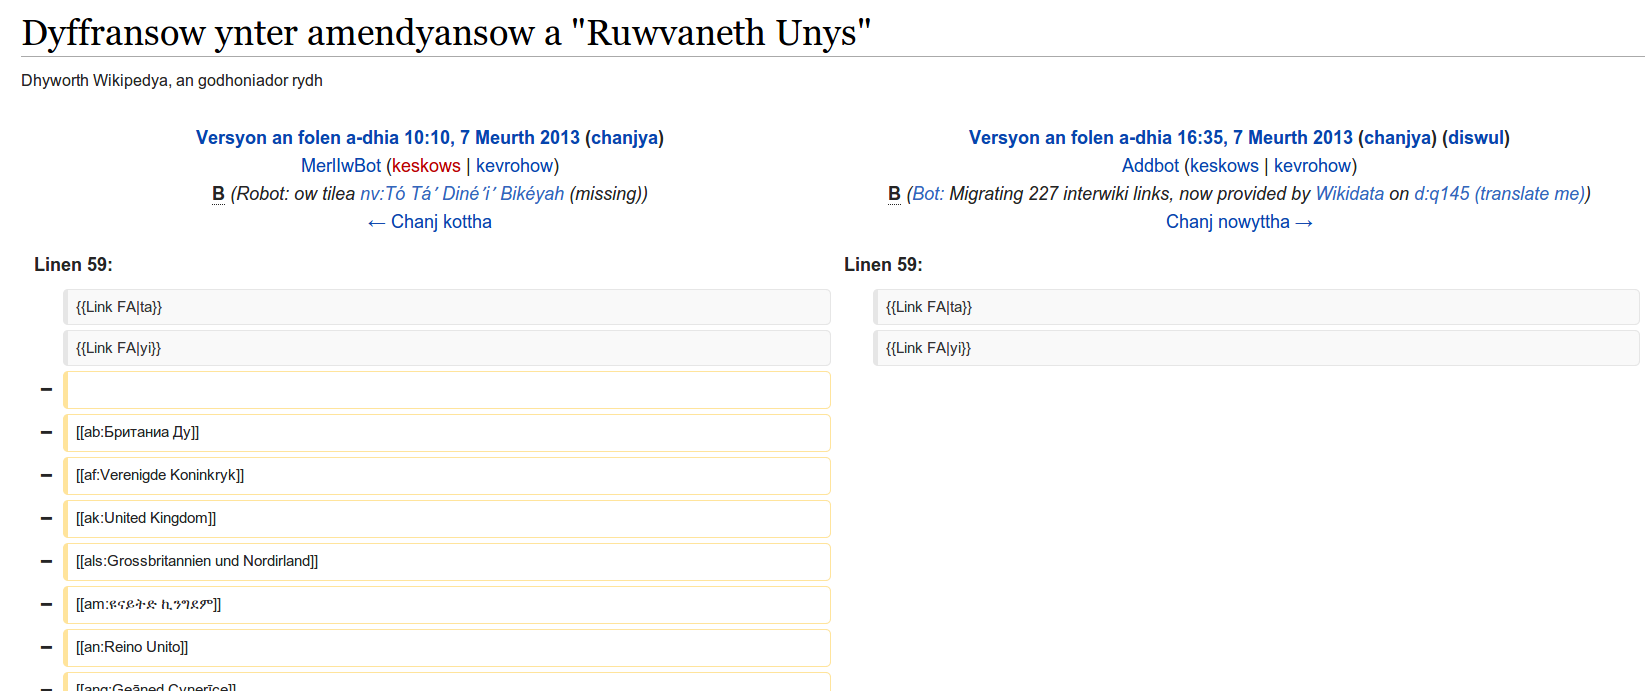
\includegraphics[width=1\linewidth]{img/traj-bot/botdiff.png}
      \caption{The Wikipedia diff for the migration event}
    \end{subfigure}
  }
\caption{Screenshots showing automated migration of inter-language links.}
\end{figure}

How do we characterise this? In this case the `article', as such, is
unchanged. Indeed the rendered page is identical before and after the
link cull. We may think to ignore bot edits to a page, but how do we
distinguish between the adding and deletion of these language links
from meaningful changes to content? We may distinguish from, say,
useful spell-checking bots by means of a simple text regex (inter-wiki
links always have the same form), but we may not as easily distinguish
language-bar links from inline ones -- those that may link to related
articles, rather than mirror articles, widening knowledge rather than
offering what may merely be a translation of the original
article.

IS THERE MORE EXAMPLE OF WEIRD WIKI STUFF MESSING UP RESULTS?

PLOT DISTRIBUTION OF EDIT NUMBER ON EN, DE, IT

PLOT DISTRIBUTION OF SPECIES OF TEXT 


\chapter{Analysis}

\section{Calculation}

The data we collect via the Wikipedia API goes through a series of
procedures in order to extract measurements of it.

%pair comparison / weighted distance
First we compare the difference between the child-parent pairs of
revisions. This process is fairly simple, and is described in
algorithm~\ref{pair-comp}. The only special condition we introduce
here is comparing the oldest revision with an empty string.

%%%%% Pair comparison algorithm
\begin{algorithm}
\caption{Pair comparison}\label{pair-comp}
  \begin{algorithmic}
    \Procedure{PairComparison}{$revids$}
    \For {$ i \gets 0, $length($revids$)}
    \If{pair distance not already in database}
    \State $str1 \gets $\LineIf{``"}{$i=0$}{database.gettext($revs[i-1]$)}
    \State $str2 \gets $database.gettext($revs[i]$)
    \State $dist \gets $PairDistance($str1, str2$)\Comment{See algorithm~\ref{dist-calc}}
    \State databaseinsert.pairdistanceinsert($dist$)  
    \EndIf
    \EndFor
  \EndProcedure
  \end{algorithmic}
\end{algorithm}

The interest, instead, is in exactly how we calculate this
distance. We discussed earlier that we would use native WikiMarkup
tags in order to identify different `species' of text. By doing so, we
could characterise a single revision in terms of the kinds of text
dealt in. By characterising an edit with a series of different edit
difference we also perhaps create the opportunity to consider some as
more valuable than others.

The algorithm that was settled upon left the levenshtein calculator
itself naive of text species -- instead we simply split the text up
and calculate levenstein distance separately. We traverse each string
from beginning to end, using simple regex expressions to identify and
extract different kinds of text, and calculating the levenshtein
distance for each separately. This process is detailed in
algorithm~\ref{dist-calc}. 

%%%%% Distance calculation procedure
\begin{algorithm}
  \caption{Revision pair distance calculation}\label{dist-calc}
  \begin{algorithmic}
    \State $regexes \gets $\{
    \Statex \tab`math1': `$<$math$>$((?!$<${\textbackslash}/math$>$).)*$<${\textbackslash}/math$>${\textbackslash}S',
    \Statex \tab`math2': `\{\{math((?!\}\}).)*\}\}',
    \Statex \tab`bquote': `$<$blockquote$>$((?!$<${\textbackslash}/blockquote$>$).)*$<${\textbackslash}/blockquote$>${\textbackslash}S'
    \Statex  \tab...
    \Statex\}\Comment{Regexes that recognise single Wikimarkup tags}
    \State $reggroups \gets $\{\label{dist-calc-groups}
    \Statex  \tab`maths':(regexes[`math1'], regexes[`math2']),
    \Statex  \tab...
    \Statex \}\Comment{Group of regexes by 'species'}
    \State $distances \gets \emptyset$
    \Function{PairDistance}{$str1,str2$}
    \State $strs \gets [str1, str2]$
    \ForAll {$key, reg \in reggroups$}
    \State $comparestr \gets [``", ``"]$
    \For {$i \gets 0,1$}
    \State $matches \gets reg.matches(strs[i])$
    \ForAll {$m \in matches$}
    \State $match, strs[i] \gets $extractsplit($m.start, m.end, strs[i]$)
    \State $comparestr[i] \gets comparestr[i] + match$
    \EndFor
    \EndFor
    \If {length($comparestr[0]$)$ > 0$ OR length($comparestr[1]$)$ > 0$}
    \State $distances[key] \gets LevDist(comparestr[0], comparestr[1])$ \Comment{See algorithm~\ref{lev-dist}}
    \Else
    \State $distances[key] \gets 0$
    \EndIf
    \EndFor
    \State $distances[$`$norm$'$] \gets LevDist(strs[0], strs[1])$
    \Comment{Process the remainder}
    \State return $distances$
    \EndFunction
  \end{algorithmic}
\end{algorithm}

In practice, this algorithm was much quicker than trying to add an
awareness of text species to the levenshtein calculator itself. We
using regex statements, we can search and split the string relatively
quickly, and use this preprocessing to alleviate the levenshtein
distance calculator of the burden of being aware of the kinds of text
it is dealing with. With this awareness integrated, because
levenshtein distance considers one character at a time, these
operations of flagging and identifying areas of text were inevitably
multiplied many thousands of time in one operation. Instead we were
able to use a fairly simply algorithm for calculating levenshtein
distance, found in algorithm~\ref{lev-dist}.

We will discuss different levenshtein-related algorithms further on
this thesis, but for now we can say that the one we reference here is
fairly basic, but with an optimised space efficiency. We see that we
don't hold a whole matrix for the two strings, only the current and
previous row. We may also describe the PairDistance overall as a
divide-and-conquer algorithm. It improves the space complexity of the
algorithm a little, and allows us the employ parallel or threaded
processing in order to improve efficiency of computation.

\begin{algorithm}
  \caption{Levenshtein distance calculator}\label{lev-dist}
  \begin{algorithmic}
    \Function{LevDist}{$str1, str2$}
    \State $s1len \gets $length($str1$)
    \State $s2len \gets $length($str2$)
    \State $column \gets [0_{1}, 0_{2}, \ldots, 0_{s1len}]$
    \For{$x \gets 1,s2len$}
    \State $col[x] \gets x$
    \EndFor
    \For{$p \gets 1,s1len$}
    \State $column[0] \gets p$
    \State $r \gets p-1$
    \For{$q \gets 1,s2len$}
    \State $oldnum \gets column[q]$
    \State $column[q] \gets min(col[q]+1, col[q-1] + 1, r + str1[p-1] \neq str2[q-1])$
    \EndFor
    \EndFor
    \State return $col[s1len]$
    \EndFunction
  \end{algorithmic}
\end{algorithm}

%%%%% Trace trajectory algorithm
\begin{algorithm}
\caption{Page trajectory calculation}\label{traj-calc}
  \begin{algorithmic}
    \Procedure{TrajectoryCalculation}{$revids, domain$}
    \State $target \gets $database.gettext($revids[-1]$)\Comment{Last revision in list is most recent}
    \For {$i \gets length(revids), 0$}
    \If{trajectory distance not already in database}
    \State $str1 \gets $database.gettext($revids[i]$)
    \State $dist \gets $LevDist($str1, target$)\Comment{See algorithm~\ref{lev-dist}}
    \State $database.inserttrajectoryinsert(dist)$    
    \EndIf
    \EndFor
    \For{$i \gets 0, length(revids)$}
    \State $dist2 \gets $database.gettrajectory($revids[i],domain$)
    \State $dist1 \gets$
        \LineIf{database.gettrajectory($revid[i-1],domain$)}{$i \neq 0$}{$2
          \times disty$}
    \State $time2 \gets $database.gettimestamp($revid[i],domain$)
    \State $time1 \gets $
        \LineIf{database.gettimestamp($revid[i-1],domain$)}{$i \neq 0$}{$timex$} 
    \State ${\Delta}x \gets time2 - time1$
    \State ${\Delta}y \gets dist2 - dist1$
    \If{${\Delta}x \neq 0$}
    \State $gradient = \frac{arctan({\Delta}y/{\Delta}x)}{\pi}$ 
    \Else 
    \State $gradient = 1$
    \EndIf
    \State database.insertgradient($revid[i],domain,gradient$)
    \EndFor
    \EndProcedure
  \end{algorithmic}
\end{algorithm}




\section{Findings}
It has been found that the population and dynamics of an online space
may affect individual user behaviour. Jones, Ravid, Rafaeli find that
Newsgroups users publish shorter posts in more populous threads.  

An interesting case is that of the english Wikipedia page on biologist
Rupert Sheldrake. Rupert Sheldrake is a biologist, who, with his
`astonishingly visionary' early work in plant science had him
described as `one of the brightest Darwinians of his
generation',\cite{odyssey-auxin}\cite{guardianshel}, came under heavy
criticism for his later work in psychical research, and `mysterious
telepathy-type interconnections between organisms and collective
memories within species'.\cite{sheldrake-biog} 

The Wikipedia article history is accordingly erratic, a continuation a
a long history of Sheldrake-bashing, as can be seen in the plots of
figure~\ref{fig:sheldrake-plots}.

\begin{figure}
  \label{fig:sheldrake-plots}
  \centering
  \makebox[\linewidth][c]{
    \begin{subfigure}[b!]{0.6\linewidth}
      \centering
      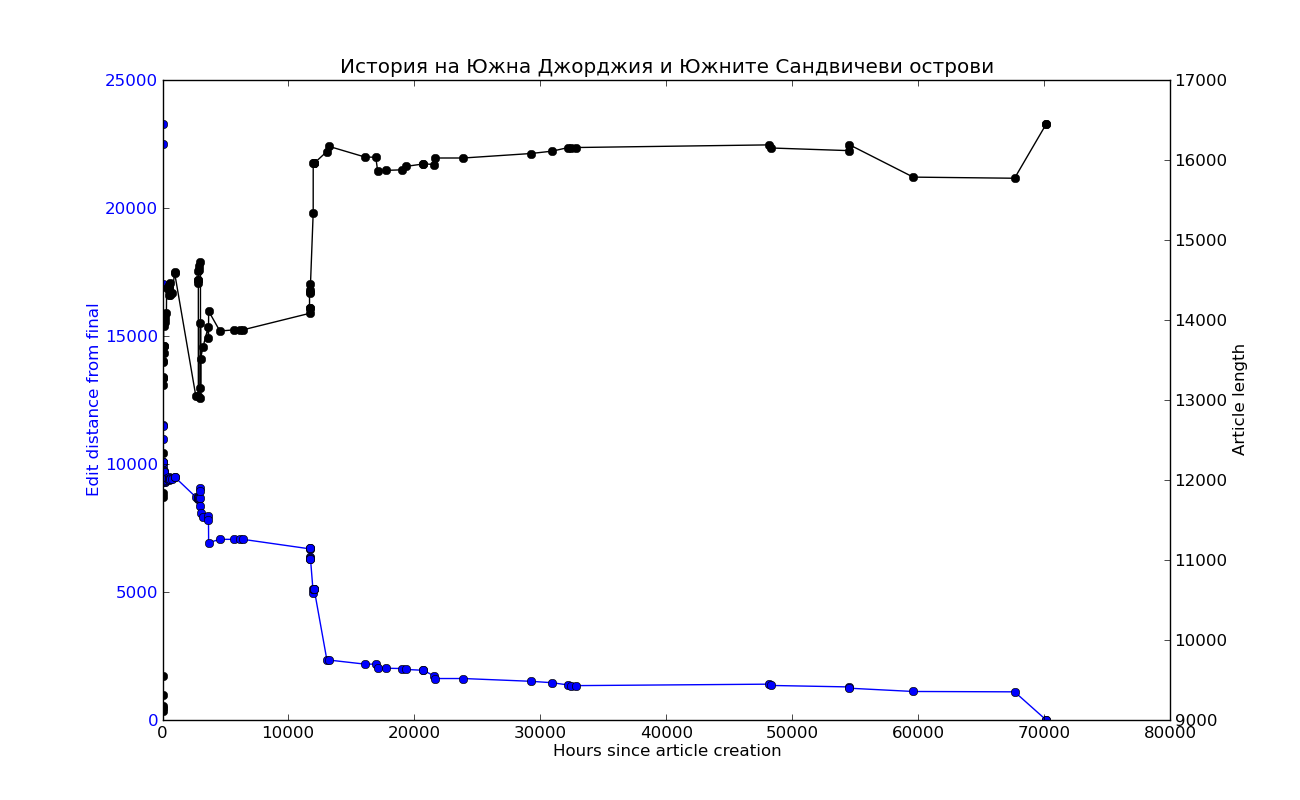
\includegraphics[width=\linewidth]{img/traj-classic/bg90882traj.png}
      \caption{\href{http://bg.wikipedia.org/wiki/index.php?curid=90882}{Bulgarian
      Wikipedia, Page ID 90882 (History of South Georgia and the South Sandwich Islands)}}
    \end{subfigure}
    \begin{subfigure}[b!]{0.6\linewidth}
      \centering
      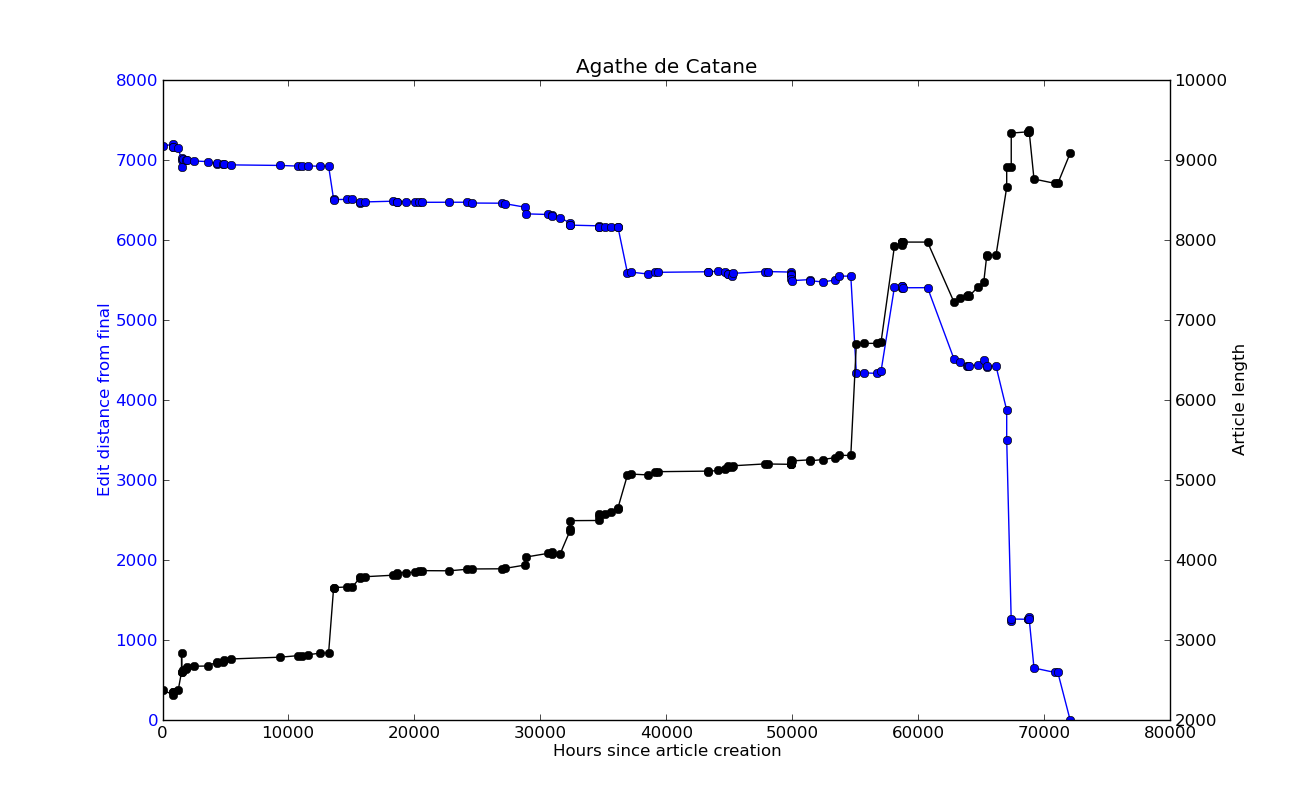
\includegraphics[width=\linewidth]{img/traj-classic/fr572796traj.png}
      \caption{\href{http://fr.wikipedia.org/wiki/index.php?curid=572796}{French
      Wikipedia, Page ID 572796 (Agatha of Catania)}}
    \end{subfigure}
  }\\
  \caption{Simple trajectory graphs.}
\end{figure}

\url{https://en.wikipedia.org/wiki/Wikipedia:Harassment#User_space_harassment}
\url{https://en.wikipedia.org/wiki/Wikipedia:Wikipedia_is_in_the_real_world}
\url{https://en.wikipedia.org/wiki/Wikipedia:Wikipedia_is_anonymous}
\url{https://en.wikipedia.org/wiki/Wikipedia:Harassment#Wikihounding}

\begin{figure}
  \begin{subfigure}[b!]{0.45\linewidth}
    \lstinputlisting[
      language=SQL,
      basicstyle=0.8\footnotesize,
      firstline=44,
      lastline=70,
    ]{results/sqlsnippet1.sql}
  \end{subfigure}
  \begin{subfigure}[b!]{0.45\linewidth}
    \lstinputlisting[
      language=SQL,
      basicstyle=0.8\footnotesize,
      firstline=71,
      lastline=97,
    ]{results/sqlsnippet1.sql}
  \end{subfigure}
  \caption{SQL snippet used to measure discrepancy between Trajectory
    calculations and distance calculations}
\end{figure}


\chapter{Evaluation}
\label{ch:evaluation}
\section{Unit testing the CLI}
We use the python `unittest' package to automate most of our
testing. The tests can be found in the package root folder in the
script `tester.py' (see appendix~\ref{sec:dirtree}).

Most of the test cases test the argParser.py logic --- the module that
checks for errors in the CLI arguments --- as most of the classes only
fail in their tasks given incorrect parameters. We also pay special
attention to the return values of each class --- in particular the
return values on failure. In our package, all exits are intended to be
handled by, and filtered up to, the wrhp.py main() function, so these
functions must fail gracefully.

\section{Evaluation of storage system}
The database was written initially to take the uniqueness of pageid
and revids for granted, but, as the project grew and we began fetching
from different language Wikipedias, the database had to change in
order to allow for duplicates of both page and revision ID, by adding
columns to all tables, and modifying their primary keys.

The database has grew organically with the project in other ways too,
and so is un-normalised. It has proven to quite robust and reliable,
but as the database grew it became quite slow. We believe it's
structure could be improved a little in order to reduce its size.

\begin{wrapfigure}{R}{0.45\linewidth}
  \begin{lstlisting}[
      basicstyle=\footnotesize,
      basicstyle=\linespread{0.8}\ttfamily,
    mathescape = true]
    P = Pageid
    T = Page title
    R = Revid
    D = Domain
    Cn = Content
    Un = Username
    Ui = Ui
    T = Revision timestampx
    S = Revision size
    Cm = Revision comment
    Mw = Math weight
    Cw = Citation weight
    Fw = Files / Images weight
    Lw = Link weight
    Sw = Structure weight
    Nw = Normal text weight
    G = Trajectory gradient
    Td = Trajectory distance
    F = Fetched flag

    RD $\rightarrow$ PMwCwFwLwSwNwCnCmGSTUnUiTd
    PD $\rightarrow$ TF
    UnD $\rightarrow$ Ui
  \end{lstlisting}
  \caption{Database fields and key dependencies}
  \label{fig:dat-key}
\end{wrapfigure}

Figure~\ref{fig:dat-key} lists the fields and key dependencies of the
database. Many of the entities of the database rely on the $(revid,
domain)$ key-pair, the only exception being the $Username, Domain
\rightarrow UserID$ and $Pageid, Domain \rightarrow Title, Fetched
flag$ relations.

Comparing this to the database schema as they stand in
figure~\ref{database-schema} we see that some improvements could be
made immediately -- the $Username, Domain \rightarrow UserID$ relation
could recieve its own schema immediately, saving a lot of repeated
information in the `wikirevisions' table. This would also be useful as
the relation could easily be expanded upon on further study into
individual user habits, as I will suggest later.

Similarly, the `title' attribute of the `wikirevisions' table could be
moved to the `wikifetched' table, since it is unique to a
$(pageid,domain)$ pair. This would necessitate the addition of a
boolean column `fetched' to the same table (the presence or lack of
presence of a given $(pageid,domain)$ pair in the `wikifetched' table
currently stands in place of that boolean value). However, given that
`wikifetched' is inevitably much smaller than `wikirevisions', the
space saved would be considerable regardless.

A further feature that can be done away with is the presence of two
revision IDs in the `wikitrajectory' table. This was useful in an
earlier implementations, where the code would manually check for both
a $(oldrevid,newrevid)$ \textit{and} $(newrevid,oldrevid)$ before
endeavouring to compute a new distance. This feature was scrubbed
early but the form of the table has survived. Similarly, content had
its own table to facilitate quicker access to revision content before
the online-viewing feature was implemented in the CLI. We could move
content to the `wikirevisions' table, safely take on the convention of
the trajectory distance being unique to either the parent or child ID,
and reduce the `wikitrajectory' table by one column.

Some structural inelegance aside, the database is fairly robust. But
given the above analysis we should recommend adoption of the schemata
described in ~\ref{fig:database-new}. Some separation of
figure~\ref{fig:dat-key}'s larger relation is recommended, to reduce
the space required, whilst keeping the some table separations for
performance and maintenance's sake. The large content table is kept
separate from the rest of the data, so as to not slow down the
database, even though a normalised database would have this data in
the wikirevisions table. Maintenance-wise, if one of the distance
calculations goes awry, for instance, one would merely have to wipe
one table and recalculate.

\begin{figure}
  \centering
  \makebox[\linewidth][c]{
    \begin{subfigure}[b!]{0.4\linewidth}
      \centering
      \begin{tabular}{ccc}
        \toprule
        \underline{username} & \underline{domain} & userid\\
        \midrule
        $\vdots$ & $\vdots$ & $\vdots$\\
      \end{tabular}
      \caption{Table: wikicontent}
    \end{subfigure}
    \begin{subfigure}[b!]{0.4\linewidth}
      \centering
      \begin{tabular}{cccc}
        \toprule
        \underline{pageid} & \underline{domain} & title & fetched? \\
        \midrule
        $\vdots$ & $\vdots$\\
      \end{tabular}
      \caption{Table: wikipages}
    \end{subfigure}
    \begin{subfigure}[b!]{0.4\linewidth}
      \centering
      \begin{tabular}{ccc}
        \toprule
        \underline{revid} & \underline{domain} & distance\\
        \midrule
        $\vdots$ & $\vdots$ & $\vdots$ \\
      \end{tabular}
      \caption{Table: wikitrajectory}
    \end{subfigure}
  }\\
  \vspace{10 mm}
  \begin{subfigure}[b!]{\linewidth}
    \centering
    \begin{tabular}{ccccccccc}
      \toprule
      \underline{revid} & \underline{domain} & pageid & username & time & size &
      comment & content \\ 
      \midrule
      $\vdots$ & $\vdots$ & $\vdots$ & $\vdots$ & $\vdots$ & $\vdots$ & $\vdots$
      & $\vdots$ & $\vdots$ \\
    \end{tabular}
    \caption{Table: wikirevisions}
  \end{subfigure}

  \begin{subfigure}[b!]{\linewidth}
    \centering
    \begin{tabular}{ccccccccc}
      \toprule
      \underline{revid} & \underline{domain} & maths & citations & filesimages & links &
      structure & normal & gradient\\
      \midrule
      $\vdots$ & $\vdots$ & $\vdots$ & $\vdots$ & $\vdots$ & $\vdots$ &
      $\vdots$ & $\vdots$ & $\vdots$ \\
    \end{tabular}
    \caption{Table: wikiweights} 
  \end{subfigure}
  \caption{Recommended new schemata for storing wikipedia data}
  \label{fig:database-new}
\end{figure}

Since, as demonstrated, we may rely on $(pageid,$ $domain)$ and
$(revid,domain)$ pairs, we are able to embed these as native psql
primary key restraints. The database will throw error `23000,
integrity constraint violation' if this restraint is threatened by the
next transaction, which is passed up from the psycopg module as an
exception.\cite{psql-error}\cite{psyc-error} If such an error occurs,
we catch it, log it, and terminate the program cleanly.

In reality, though, these errors are infrequent. The code only
prepares and inserts a value if it cannot find it in the database, and
the insertion functions are implemented as to check before inserting
that it will not be duplicating any data.

\subsection{Logging}
We implement basic but thorough info and debug logging throughout the
program. 
I log.


\section{Machine learning validation attempts}
\label{mlisbad}
We attempted to validate our model using machine learning. Given the
form of the model's output -- a 1D array of numbers -- machine
learning seemed to be a natural choice.

We were interested to see if we could predict gradient factor. Since
the gradient factor relates closely to whether or not the edit was
included in the final version, we were interested if with machine
learning could possibly predict the gradient factor given the weights
that we calculate. We could possibly see if the text analysis data we
had collected would be able to similarly measure affects on the
article.

We used the scikit-learn python package to approach the
problem,~\ref{scikit-learn} working with the ~180,000 test cases (i.e.
complete revision records) extant in the database at the time. We
tried predicting gradient factor with the following forms of training
data:

\begin{itemize}
  \item \textbf{Weights}\\
    Simply the calculated weights, as found in the database weight table. 

  \item \textbf{Weights and size change}\\
    The calculated, along with information about whether the revision
    made the article larger or smaller

  \item \textbf{Weights size change, time change}\\
    The calculated, along with information about whether the revision
    made the article larger or smaller

  \item \textbf{Weights summed to one value, and size change}\\
    Summing the weights to one value is roughly equivalent to taking a
    plain levenshtein distance of the article on the whole, rather
    than one separated by species.
    
  \item \textbf{Summed weights and user edit count over
    domain}\\ We take the generic weight and combine it with the
    user's activity over the whole wikipedia domain.
    
  \item \textbf{Summed weights and user edit count over
    article}\\ Similar to above, but only counts user activity in the
    same article.

\end{itemize}

We experimented with various types of regression techniques, but our
results were not very good, with the regression function rarely
fitting to the data with any accuracy. The validation scripts can be
run from validator.py, in the validation sub-folder.

Since the gradient factor is sensitive to time, and the scale of that
time, we also tried separating the data into two categories,
'towards-final' as 1 and 'away-from-final' as 0, by simply rounding
the gradient factor to it's nearest integer, and repeated the same
tests as detailed above, but similarly the classification was not very
accurate.

We identify two problems that may have effected this. 

Our first is perhaps the incompleteness of our data. In particular,
the incompleteness of our understanding of the text itself. It was a
central premise of this study that we were to make no attempt at
understanding the actual content of the text.

But perhaps the actual fact content of the text is quite important,
particularly on an encyclopaedia, to its survival --- perhaps Wikipedia
is predictable in this regard, that facts have an innate discoverable
quality. Perhaps in this case we would be in a better place to predict
success if we could measure the factual accuracy of new text, run a
spell checks on it, etc.

Our second problem may be that, perhaps, much of the data we analysed
actually doesn't greatly effect the survival rate of the edit. Much of
the information lost from and gained by pages like Rupert Sheldrake's,
or Derek Smart's was factually correct, and not necessarily
malformed. The reason for the exclusion of content was to quell a
conflict in the case of the former text, whereas in the latter page it
was the personal opinions of individual Wikipedia editors about which
facts actually \text{were} facts that caused (and continue to cause)
complications.

Talk page data is one thing, and we looked briefly at how the talk
page data can correlate with article data, but external context is
relevant too. Rupert Sheldrake's interview on the BBC coincides with
changes in his article, and we can refer to Lih's 2004 article on
edits made immediately after celebrity deaths.

We note that there are less regular editors on Wikipedia now than
there was in 2007, user-count `has shrunk by more than a third since
[then] and is still shrinking'.\cite{wiki-decline} Wikipedia's `formal
mechanisms for normal articulation are shown to have calcified against
changes –-- especially changes proposed by newer
editors'.\cite{wiki-decline-2} The study identifies, amongst other
things, a number of tools, bots and policies that have often tended to
revert entries regardless of their content.

But Wikipedia's internal problems are of not real issue with this
study, they only give us reason to doubt whether we could use a simple
dataset in order to characterise the complex conditions that conduce a
successful contribution to Wikipedia.

Rather, the lesson we learn here is simply that a wide context is
necessary for understanding and characterising real-world human
collaboration.


\chapter{Conclusion}
\label{ch:conclusions}
\section{Summary of Thesis Achievements}
We have looked into the possibility towards the idea of quality in
Wikipedia. 

We saw that many MANY studies use many seemingly arbitrary means to
find GOOD in a wikipedia.

We wanted something more generic. There were studies that used less
arbitrary means. CITE crowdsourced WikiVandalism corpus. 

So we considered looking at the current point of an article to be a
kind of culmination point. This seemed appropriate for Wikipedia's
philosophy. See quote. But also for the nature of knowledge itself --
we learn new things, we incorporate them. A conclusion can keep being
added to.

ALSO MAYBE just maYBE an article has value in the past. but we're not
there.

In the end we are seemingly brought to the conclusion that naive
textual analysis does not affect survival rate of text -- there are
simply too many contextual factors governing it. From our failure to
find correlation between our gradient factor and our other dat (see
section~\ref{mlisbad}), we may begin to conclude that text type isn't
innately connected to 

So, with our automatically we are unable to predict the shape of the
trajectory graph until the entire history is fetched. Does that mean
this is a failure? 

There is a hope we can predict success on edit count, `seniority' of
editor. We could perhaps analyse the edit with awareness, looking for
corroboration online with the information contained in the
text. Way beyond the scope of this project, but possible.

However, we can't predict the future. And if we can predict the
edit-power of an editor, we can't necessarily predict his opinion. Or
even his mood at the time of editing. Refer to Rupert Sheldrake.

\section{Applications}
The software, as it stands, provides a fairly open and malleable
source for examining the histories of Wikipedia articles. As a
history-visualisation tool, it is different to existing tools (the
most comparable is IBM's blah, though it is more concerned about the
history of each section of a wikipedia article) in that allows for
more flexibility in analysing pages. We have shown how it may also be
leveraged to combine plots of different pages, to allow for greater
context.

The modularity of the approach also allows for more radical changes to
the software. The project could be easily adapted to handle different
data, with little change. To handle GitHub document history, merely
changing the database wrapper and API wrapper classes could be enough
to begin analysing the data there. The anlaysing class asks for text
content based on a two unique identifier -- the file ID and the
revision ID. The trajectory graph, for instance, could be plotted
without trouble.

IF HAVE TIME ACTUALLY DO THAT JUST FOR A SECOND, of the analysing
class. Lolz.

\section{Summary}
Wikipedia proved to be a good case study for the exploring how we may
automatically analyse an individual's collaborative stake in a joint,
text based work.

It is perhaps one of the most interesting parts of Wiki analysis that
evidence such interpersonal acts is so readily available. Due to the
nature of the WikiMedia software, these interactions are as publicly
available as the article's themselves, all utilising the same text
revision framework. Through this we were able to expand our knowledge
of the circumstance of the collaboration, and by proxy our
understanding of each collaborative act, using one set of tools.

Our conclusions are ambiguous. As this work stands, building upon the
work of the previous year to achieve an automatic and expandable
framework for analysis, it makes a healthy attempt at describing each
edit in terms of it's input. We may even describe our weighted
levenshtein distance calculator to be a lossy compression algorithm,
reducing the text down to its meaningful parts.

However, our second measure, gradient factor, which describes both the
local and long-term success of a revision did not seem to correlate
well with the above measure.

We acknowledge that na\"ive string analysis, by definition, excludes
the recognition of quality content in terms of facts, well-formedness,
and so on. These qualities affect the result of a collaborative act,
of course, particularly when contributing to a knowledge
repository. But we also acknowledge that the correlation between edit
content and edit success may not have a simple correlation.

For all the studies that sought out to analyse objective quality in
articles, and edits, there are also studies of Wikipedia's biased
attitudes to what edits may stay in an article. The part of our study
that concerned talk-pages and arbitration requests contributed to the
latter line of enquiry.

And we believe that this may not merely be a problem native to
Wikipedia, or on-line discourse. We believe that Wikipedia may merely
present a more-than-usually analysable trace of the inter-personal
relations that shape all collaborations. In some of the cases
described here these interactions are evidenced in talk-page
communication. In others, like in undo-redo edit wars, the interaction
is embedded in the act of editing itself. 

And this is not to mention the myriad external factors that also
affect regard to individual edits --- long-standing off-Wikipedia
arguments in both the Rupert Sheldrake and Derek Smart articles
referred to previously. Again, with search engines we have the
opportunity to track these waves of opinion, complex changes in the
standard of knowledge of that occur naturally. 

But the individual predilections of key, more active editors, if not
evidenced in previous edits, remain a mystery. As may, of course, the
habits and opinions of a manger in a group-coding scenario --- until
they are codified in action.

The lesson we learn overall, then, is that if we can't predict the
fore-coming trajectory of an article, we may certainly have the means
to analyse it once the fact of the history of the article is
crystallised. We achieved this by deciding the article was
conceptually `finished' at the most recent revision we fetch. The
`finished' state is in other collaborative platforms.

If surrounding context as important as it seems in this study, then we
have learnt a user's stake in a collaborative work should be as
affected by the degree of discussion and coordination that that
individual engaged as it is by actual evidenced output.

In the chaos of on-line interaction that characterises Wikipedia, we
must look not only to the final work. We must take into account
measures of interaction, and a users weight in the overall community
network of the on-line space. Their valuable contributions are not only
factual, but social; the collaboration is not merely the sum of its
parts, but also product of a community, a network, and a society.  

%% one
%% of the most popular websites in the world, we find that other factors
%% are more correlated with survival -- factors incident to to the nature
%% of the Wikipedia `community', and a user's place within that
%% community, rather than the content of the edit itself.

%% We have looked into the possibility towards the idea of quality in
%% Wikipedia. 

%% We saw that many MANY studies use many seemingly arbitrary means to
%% find GOOD in a wikipedia.

%% We wanted something more generic. There were studies that used less
%% arbitrary means. CITE crowdsourced WikiVandalism corpus. 

%% So we considered looking at the current point of an article to be a
%% kind of culmination point. This seemed appropriate for Wikipedia's
%% philosophy. See quote. But also for the nature of knowledge itself --
%% we learn new things, we incorporate them. A conclusion can keep being
%% added to.

%% ALSO MAYBE just maYBE an article has value in the past. but we're not
%% there.
%% -
%% In the end we are seemingly brought to the conclusion that naive
%% textual analysis does not affect survival rate of text -- there are
%% simply too many contextual factors governing it. From our failure to
%% find correlation between our gradient factor and our other dat (see
%% section~\ref{mlisbad}), we may begin to conclude that text type isn't
%% innately connected to 

%% So, with our automatically we are unable to predict the shape of the
%% trajectory graph until the entire history is fetched. Does that mean
%% this is a failure? 

%% There is a hope we can predict success on edit count, `seniority' of
%% editor. We could perhaps analyse the edit with awareness, looking for
%% corroboration online with the information contained in the
%% text. Way beyond the scope of this project, but possible.

%% However, we can't predict the future. And if we can predict the
%% edit-power of an editor, we can't necessarily predict his opinion. Or
%% even his mood at the time of editing. Refer to Rupert Sheldrake.


%% INSERT THING ABOUT GOOGLE POPULAR THING

%% In the world of physical collaboration these kind of interpersonal
%% artefacts of cooperation are apparent. With wikipedia we get a clearly
%% traceable stuff.

%% PLOT DISTRIBUTION OF EDIT NUMBER ON EN, DE, IT

%% PLOT DISTRIBUTION OF SPECIES OF TEXT 

%% THE CASE FOR STUDYING NETWORK 

%% --Frederick Chopin + talk
%% --Rupert Sheldrak + talk
%% --Derek Smart + talk
%% --Aluminium + talk

%% \url{https://en.wikipedia.org/wiki/Wikipedia:Harassment#User_space_harassment}
%% \url{https://en.wikipedia.org/wiki/Wikipedia:Wikipedia_is_in_the_real_world}
%% \url{https://en.wikipedia.org/wiki/Wikipedia:Wikipedia_is_anonymous}
%% \url{https://en.wikipedia.org/wiki/Wikipedia:Harassment#Wikihounding}


\appendix

\begin{appendices}
\chapter{Guide to code base}
\label{sec:dirtree}
\dirtree{%
.1 /wikiInterface.
.2 \_\_init\_\_.py.
.2 consts.py.
.2 wrhp.py \quad $\triangleleft$ the base CLI main().
.2 argParser.py.
.2 wikiDataHandle.py.
.2 wikiDataPlot.py.
.2 wikiAnalysis.py \quad $\triangleleft$ analytical methods. 
.2 launch.py \quad $\triangleleft$ opens wikipedia pages in default browser.
.2 logger.py \quad $\triangleleft$ shared logging functions.
.2 info.log \quad $\triangleleft$ info log destination.
.2 debug.log \quad $\triangleleft$ debug log destination.
.2 unittests.py \quad $\triangleleft$ unit testing scripts.
.2 dbpas.
.2 lshtein \quad $\triangleleft$ the levenshtein calculator files.
.3 \_\_init\_\_.py.
.3 fastlev.so.
.3 fastlev.
.4 fastlev.cpp. 
.4 setup.py.
.4 Makefile.
.2 scraper.
.3 wikiRevisionScrape.py. 
.3 \_\_init\_\_.py.
.3 langs.csv \quad $\triangleleft$ details of different language wikipedias.
.2 database.
.3 \_\_init\_\_.py.
.3 wikiData.py \quad $\triangleleft$ database wrapper.
.3 schemamake.sql \quad $\triangleleft$ database schema definitions.
.2 validate \quad $\triangleleft$ the validation / testing scripts.
.3 validator.py.
}

\end{appendices}

\phantomsection
\addcontentsline{toc}{chapter}{Bibliography}
\printbibliography        


\end{document}
